\documentclass{beamer}

\setbeamerfont{footnote}{size=\tiny}
\AtBeginSection[]
{
  \begin{frame}<beamer>
%    \frametitle{Outline for Section \thesection}
    \frametitle{Outline (Redux)}
    \tableofcontents[currentsection]
  \end{frame}
}
\usepackage{tikz}

\usetheme{CambridgeUS}
\setbeamercolor{title}{bg=red!65!black,fg=white}

\setbeamertemplate{sidebar right}
{
  \vfill%
  \llap{\insertlogo\hskip0.1cm}%
  \vskip2pt%
  \llap{\href{http://domdisanto.github.io}{Downloadable Slides}\hskip0.2cm}% NEW
  \vskip3pt% NEW
  \llap{\usebeamertemplate***{navigation symbols}\hskip0.1cm}%
  \vskip2pt%
}


% Bibliography Options 
\usepackage[url=false, doi=false, maxcitenames=1, isbn=false]{biblatex}
\addbibresource{BST245_Project.bib}

\title{Graphical Models}
\subtitle{With a focus towards interimly missing data}
\author{Dominic DiSanto}
\institute[]{Department of Biostatistics, Harvard University}
\date{\today}


% Custom commands 
\newcommand{\nhood}{\text{ne}}

%%%%%%%%%%%%%%%%%%%%%%%%
    % START %%%%%%%%%%%%
%%%%%%%%%%%%%%%%%%%%%%%%
\begin{document}

\begin{frame}{Notes (To Be Deleted)}
    \begin{itemize}
        \item Maybe scrap nhood selection for time 
        \item \textcolor{red}{Be able to speak to glasso over neighborhood selection, how sparsity guarantees MLE existence}
        \item Analyses/slides for missingness TBD 
    \end{itemize}
\end{frame}


\maketitle


\begin{frame}{Outline}
\tableofcontents 
\end{frame}

\begin{frame}{Disclaimers}
    \begin{itemize}\setlength\itemsep{8mm}
        \item Historical coverage is to the best of my ability and time constraint, please correct me with additional information
        \item Interrupt with any questions, clarification, confusion, etc. 
        \item This is far from a comprehensive treatment, but I attempt to be holistic in my coverage 
    \end{itemize}
\end{frame}

\iffalse 
\begin{frame}{Goals}
    \begin{itemize}\setlength\itemsep{8mm}
        \item Introduce random graphs as (useful) representations of multivariate, random data
        \item Outline useful methods and shortcomings in "typical" analysis (read: ideal data) of graphical models 
        \item Orient you to 
    \end{itemize}
\end{frame}
\fi 

\section{Introduction to Graphical Models}

\begin{frame}{Graph Theory Origins \cite{imperatorskaia_akademia_nauk_russia_commentarii_1726,shields_cultural_2012}}
\begin{figure}
    \centering 
    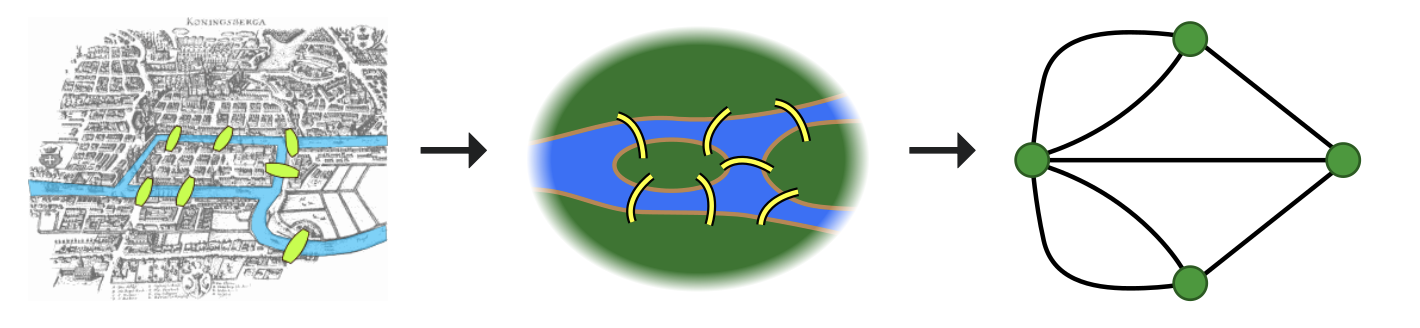
\includegraphics[scale=0.5]{Wikipedia_Bridges.png}
    \caption{Euler's Bridges Conceptualization (Recreation)}\footnote{Image taken from Wikipedia (\url{https://en.wikipedia.org/wiki/Seven_Bridges_of_Konigsberg})}
\end{figure}
\end{frame}


%\section*{Historical Notes}

\begin{frame}{Early Applications of Graphs in Mathematics}
\begin{itemize}
    \item Graph theory attributed to begin with Euler and the "Seven Bridges of K\"onigsberg" ($\sim$1736)
    \pgfsetfillopacity{0.4}
    \item Random graph theory began developing in $\sim$1940's (Moreno and Jennings) but most notably with the Erd\"os-R\'enyi random graph (1958)
    \item Ising model ($\sim$1920's) - proposed graphical model of interactions of atomic spin
    \item Statistical "beginnings"%\footnote{"Beginnings" as earlier applications in physics were probabilistic by construction, but this may be seen as the earliest application purely from a statistical point of view, i.e. without considering physical phenomena} as a subset of methods for contingency tables and log-linear models ($\sim$1970's)
    \item Arthur Dempster (founding Harvard Stats professor) introduced covariate selection by precision matrix estimation in 1972 \cite{dempster_covariance_1972}
    \item Judea Pearl $\sim$1980's for causal intepretation of Bayesian networks
    \item Modern interest in related regularized M-estimation problems and graphical neural networks 
\end{itemize}
\end{frame}
\pgfsetfillopacity{1}


\begin{frame}{Early Applications of Graphs in Mathematics}
    \begin{itemize}
        \pgfsetfillopacity{0.4}
        \item Graph theory attributed to begin with Euler and the "Seven Bridges of K\"onigsberg" ($\sim$1736)
        \item Random graph theory began developing in $\sim$1940's (Moreno and Jennings) but most notably with the Erd\"os-R\'enyi random graph (1958)
        \pgfsetfillopacity{1}
        \item Ising model ($\sim$1920's) - proposed a graphical model of interactions of atomic spin
        \pgfsetfillopacity{0.4}
        \item Statistical "beginnings"%\footnote{"Beginnings" as earlier applications in physics were probabilistic by construction, but this may be seen as the earliest application purely from a statistical point of view, i.e. without considering physical phenomena} as a subset of methods for contingency tables and log-linear models ($\sim$1970's)
        \item Arthur Dempster (founding Harvard Stats professor) introduced covariate selection by precision matrix estimation in 1972 \cite{dempster_covariance_1972}
        \item Judea Pearl $\sim$1980's for causal intepretation of Bayesian networks
        \item Modern interest in related regularized M-estimation problems and graphical neural networks 
    \end{itemize}
    \end{frame}



\begin{frame}{Early Applications of Graphs in Mathematics}
    \begin{itemize}
        \pgfsetfillopacity{0.4}
        \item Graph theory attributed to begin with Euler and the "Seven Bridges of K\"onigsberg" ($\sim$1736)
        \item Random graph theory began developing in $\sim$1940's (Moreno and Jennings) but most notably with the Erd\"os-R\'enyi random graph (1958)
        \item Ising model ($\sim$1920's) - proposed a graphical model of interactions of atomic spin
        \pgfsetfillopacity{1}
        \item Statistical "beginnings"\footnote{Early use in physics were probabilistic, but this may be seen as an early "purse statistics" application} as a subset of methods for contingency tables and log-linear models ($\sim$1970's)
        \pgfsetfillopacity{0.4}
        \item Arthur Dempster (founding Harvard Stats professor) introduced covariate selection by precision matrix estimation in 1972 \cite{dempster_covariance_1972}
        \item Judea Pearl $\sim$1980's for causal intepretation of Bayesian networks
        \pgfsetfillopacity{1}
        \item Modern interest in related regularized M-estimation problems and graphical neural networks 
    \end{itemize}
\end{frame}
    \pgfsetfillopacity{1}



\begin{frame}{Graphical Model Motivation}
    \begin{columns}[T]
        \begin{column}{0.6\textwidth}
            Suppose you have 20 random variables$^*$, how do you model their interrelationship? \newline 
            \vspace{2mm}
            $^*$Consider any of the following:
            \begin{itemize}
                \setlength
            \item General -omic data
            \item Spatial data 
            \item Computational neuroscience data 
            \item Clinical language (see: EHR LLM\footnote{Electronic Healthcare Record Large Language Model})
            \item Time-series data 
            \end{itemize}
        \end{column}
        \begin{column}{0.4\textwidth}
        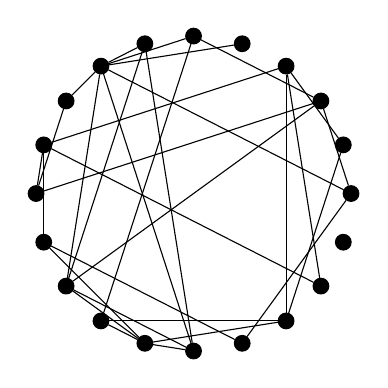
\begin{tikzpicture}
            \foreach \i in {1,...,20} {
                \node[circle, draw, fill=black, inner sep=2pt] (node\i) at ({360/20 * (\i - 1)}:2) {};
              }
            
              \foreach \i in {1,...,19} {
                \foreach \j in {\i,...,20} {
                  \ifnum\i<\j
                    \pgfmathparse{rnd}
                    \ifdim\pgfmathresult pt<0.15pt
                      \draw (node\i) -- (node\j);
                    \fi
                  \fi
                }
              }
            \end{tikzpicture}      
        \end{column}
    \end{columns}
\end{frame}


\begin{frame}{Graphs}
    \begin{itemize}\setlength\itemsep{4mm}
        \item Graphs are a natural way to represent interrelationships among our data! 
        \item Present nice properties for estimation of joint distributions 
        \begin{itemize}
            \item Can avail existing graphical algorithms
            \item Ability to characterize conditional (in)dependencies
        \end{itemize}
        \item Probabilistic graphical modelling provide a general formalism of many existing methods in statistics (e.g. Bayesian hierarchical modelling, Hidden Markov Models, Kalman filter)
        % BHM's can be represented by a DAG, hence yielding available directed methods 
        % HMM's (which are a specific dynamic Bayesian network) , see https://www.cs.ubc.ca/~murphyk/Bayes/bayes.html
        \item Wainwright, Jordan {\it "Graphical Models, Exponential Families, and Variational Inference"} (2007) is an excellent reference for further applications (and theory) behind graphical models \cite{wainwright_graphical_2007}\footnote{See 2.4 specifically for applications}
    \end{itemize}
\end{frame}

\begin{frame}{Graphs}
    \begin{columns}[T] % align columns at the top
        \begin{column}{.7\textwidth}
            \begin{itemize}%{.5\textwidth}
                \setlength\itemsep{5mm}
                \item Consider random vector $X \sim N(\boldsymbol\mu, \Sigma)$ and precision matrix $\Theta \equiv \Sigma^{-1}$
                \begin{itemize} 
                    \item Interested in estimating $\Sigma$ to characterize joint distribution $f_X$
                \end{itemize}
                \item Can construct a resulting graph $\mathcal{G} = (V, E)$, $V = X, E \subseteq V \times V$
                \begin{itemize} \item Let $\nhood(x)$ represent the neighborhood of $x$, or $\nhood(x) = \{b \in V \mid (x,b) \in E\}$ \end{itemize}
                \item Can construct adjacency matrix $A \in \mathbb{R}^{|V| \times |V|}$ describing edge set $E$ 
                    \begin{itemize} 
                        \item $A_{ij}=\mathbb{I}\{(i,j) \in E\}$ 
                        \item Let $D_{max}$ represent the maximum degree
                    \end{itemize} 
                \end{itemize}
        \end{column}
        \begin{column}{.3\textwidth}
            %\begin{figure}
                \centering
            \scalebox{0.9}{
                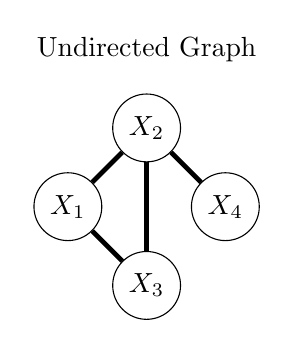
\begin{tikzpicture}
                \node[circle, draw] (A) at (0,0) {$X_1$};
                \node[circle, draw] (B) at (1,1) {$X_2$};
                \node[circle, draw] (C) at (1,-1) {$X_3$};
                \node[circle, draw] (D) at (2,0) {$X_4$};
                \node[] (capt) at (1, 2) {Undirected Graph};
                \draw[line width=0.6mm] (A) -- (B);
                \draw[line width=0.6mm] (A) -- (C);
                \draw[line width=0.6mm] (B) -- (D);
                \draw[line width=0.6mm] (C) -- (B);
            \end{tikzpicture}
            }
            %\caption{Undirected Graph}
            %\end{figure}
            \\ \vspace{3mm}
            \scalebox{0.9}{
            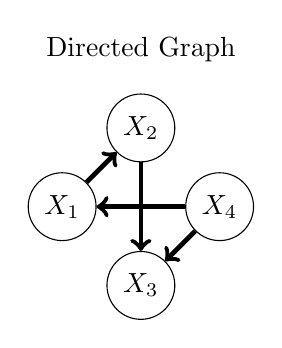
\begin{tikzpicture}%[opacity=0.2]
                \node[circle, draw] (A) at (0,0) {$X_1$};
                \node[circle, draw] (B) at (1,1) {$X_2$};
                \node[circle, draw] (C) at (1,-1) {$X_3$};
                \node[circle, draw] (D) at (2,0) {$X_4$};
                \node[] (capt) at (1, 2) {Directed Graph};
                \draw [line width=0.6mm, ->]
                    (A) edge (B)
                    (D) edge (A) 
                    (D) edge (C) 
                    (B) edge (C);
            \end{tikzpicture}
            }
        \end{column}
    \end{columns}
\end{frame}


\begin{frame}{Notation/Nomenclature}{\it Omitting some philosophical discrepancies}
    \begin{itemize}
        \item Directed (Acyclic) Graph $\Leftrightarrow$ Bayesian network
        \vspace{10mm}
        \item Undirected graph $\Leftrightarrow$ Markov network / Markov random field
    \end{itemize}
\end{frame}


\begin{frame}{Graphs}
    \begin{columns}[T] % align columns at the top
        \begin{column}{.7\textwidth}
            \begin{itemize}%{.5\textwidth}
                \setlength\itemsep{5mm}
                \item Consider random vector $X \sim N(\boldsymbol\mu, \Sigma)$ and precision matrix $\Theta \equiv \Sigma^{-1}$
                \begin{itemize} 
                    \item Interested in estimating $\Sigma$ to characterize joint distribution $f_X$
                \end{itemize}
                \item Can construct a resulting graph $\mathcal{G} = (V, E)$, $V = X, E \subseteq V \times V$
                \begin{itemize} \item Let $\nhood(x)$ represent the neighborhood of $x$, or $\nhood(x) = \{b \in V \mid (x,b) \in E\}$ \end{itemize}
                \item Can construct adjacency matrix $A \in \mathbb{R}^{|V| \times |V|}$ describing edge set $E$ 
                    \begin{itemize} 
                        \item $A_{ij}=\mathbb{I}\{(i,j) \in E\}$ 
                        \item Let $D_{max}$ represent the maximum degree 
                    \end{itemize}
                \end{itemize}
        \end{column}
        \begin{column}{.3\textwidth}
            %\begin{figure}
                \centering
            \scalebox{0.9}{
                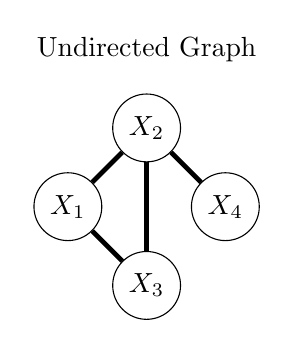
\begin{tikzpicture}
                \node[circle, draw] (A) at (0,0) {$X_1$};
                \node[circle, draw] (B) at (1,1) {$X_2$};
                \node[circle, draw] (C) at (1,-1) {$X_3$};
                \node[circle, draw] (D) at (2,0) {$X_4$};
                \node[] (capt) at (1, 2) {Undirected Graph};
                \draw[line width=0.6mm] (A) -- (B);
                \draw[line width=0.6mm] (A) -- (C);
                \draw[line width=0.6mm] (B) -- (D);
                \draw[line width=0.6mm] (C) -- (B);
            \end{tikzpicture}
            }
            %\caption{Undirected Graph}
            %\end{figure}
            \\ \vspace{3mm}
            \scalebox{0.9}{
            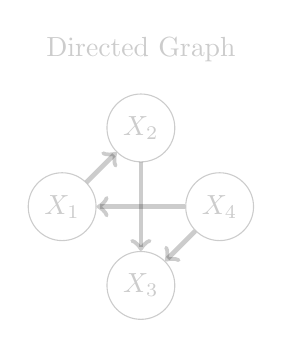
\begin{tikzpicture}[opacity=0.2]
                \node[circle, draw] (A) at (0,0) {$X_1$};
                \node[circle, draw] (B) at (1,1) {$X_2$};
                \node[circle, draw] (C) at (1,-1) {$X_3$};
                \node[circle, draw] (D) at (2,0) {$X_4$};
                \node[] (capt) at (1, 2) {Directed Graph};
                \draw [line width=0.6mm, ->]
                    (A) edge (B)
                    (D) edge (A) 
                    (D) edge (C) 
                    (B) edge (C);
            \end{tikzpicture}
            }
        \end{column}
    \end{columns}
\end{frame}





\begin{frame}{How do we estimate graph structure?}
    \centering
    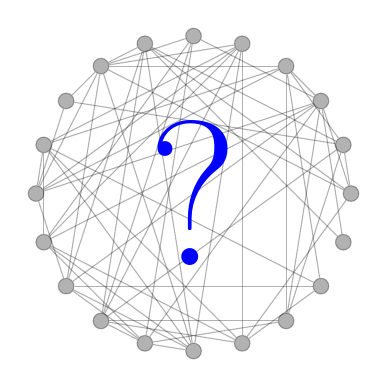
\begin{tikzpicture}[opacity=0.3]
        \foreach \i in {1,...,20} {
            \node[circle, draw, fill=black, inner sep=2pt] (node\i) at ({360/20 * (\i - 1)}:2) {};
          }
        
          \foreach \i in {1,...,19} {
            \foreach \j in {\i,...,20} {
              \ifnum\i<\j
                \pgfmathparse{rnd}
                \ifdim\pgfmathresult pt<0.3pt
                  \draw (node\i) -- (node\j);
                \fi
              \fi
            }
          }
    \node[blue, scale=3, opacity=1] at (0,0) {\Huge ?}; % Add a large question mark in the center
    \end{tikzpicture}
\end{frame}

\begin{frame}{Gaussian Graphical Models}
    Recall the form and properties of a multivariate Gaussian random vector:
    \begin{gather*}
        f(x; \mu, \Theta) = \frac{1}{(2\pi)^{d/2} |\Theta|^{1/2}} \exp\left(-\frac{1}{2} (x - \mu)^T \Theta (x - \mu)\right)
    \end{gather*}

\[
\mathbb{E}[X_i \mid X_{(-i)}] = \mu_i + (X_{(-i)} - \mu_{(-i)})^T \Theta_{j \neq i} \sigma_{i, j\neq i}
\]

\[
\text{Var}[X_i \mid X_{(-i)}] = \Sigma_{ii} - \sigma_{i, j \neq i}^T \Theta_{j \neq i} \sigma_{j \neq i, i}
\]

\end{frame}



\begin{frame}{Gaussian Graphical Models}

{\bf Gaussianity gives us the nice property that $\Theta_{ij}=0 \Leftrightarrow X_i \perp X_j | X_{-\{i,j\}}$ }

\[
\mathbb{E}[X_i \mid X_{(-i)}] = \mu_i + (X_{(-i)} - \mu_{(-i)})^T \Theta_{j \neq i} \sigma_{i, j\neq i}
\]

\[
\text{Var}[X_i \mid X_{(-i)}] = \Sigma_{ii} - \sigma_{i, j \neq i}^T \Theta_{j \neq i} \sigma_{j \neq i, i}
\]

\end{frame}



\section{Estimation for Complete Data}

\subsection{Neighborhood Selection}

\begin{frame}{Preface}
    \begin{itemize}\setlength\itemsep{6mm}
        \item Consider the setting of graph estimation for $X = (X_1, ..., X_d)$
        \begin{itemize} \item Generally your data may or may not contain a "response variable" of interest \end{itemize}
        \item Identifying conditional relationships $\Leftrightarrow$ Estimating/Identifying 0's in $\Sigma$
        \item Enforse sparsity for $\hat\Theta$ to account for possible rank-degeneracy of $S$ if $d \gg N$
        % in fact, under p \leq N the \Theta MLE can still exhibit \cite{mazumder_graphical_2012}
        %\item Exhaustive search is quickly infeasible, but can yield solutions with theoretical guarantees
        %\begin{itemize} \item Consistency \item Nice statistical rates \end{itemize}
        %\item Far from exhaustive, these methods are nice for 
        %\begin{itemize} 
        %    \item $\ell_1$ peantly 
        %\end{itemize}
        % EDIT be able to discuss more intelligently
    % Talk about what consistency means and a nice rate means for graphical models here (maybe another slide to be most explicit but TBD)
    \end{itemize}
\end{frame}

\begin{frame}{Neighborhood Selection}
    \begin{itemize}\setlength\itemsep{6mm}
        \item Note that $E \backslash \{\nhood(X_i)\}$ includes all nodes independent of $X_i$ conditional upon $\nhood(X_i)$
        \item Proposed by Meinshausen \& B\"uhlmann (2006) \cite{meinshausen_high-dimensional_2006}, for $X\in\mathbb{R}^d$ concern yourself only with $(\Theta)_{ij} =0,$ or $(\Theta)_{ij}\neq 0$
        \item Assume sparsity of $\Theta$ and fit $d$, element-wise lasso models 
        \begin{itemize}
            \item Regress $X_i \stackrel{\text{Lasso}}{\sim} X_1 + ... X_{i-1} + X_{i+1} + ... + X_d$ for all $i\in [d]$
            \item Take $\hat\beta_{(-i)} \in \mathbb{R}^{d-1}$ from each model
            \item Conclude\footnote{Authors both AND or OR rule for final step with similar performance} $(\Theta)_{ij} = 0 \Leftrightarrow \hat\beta_{(-i)j} = 0 \land \hat\beta_{(-j)i}=0$
        \end{itemize}
        \item Admits asymptotic consistency for "zero-selection" of $\Theta$
    \end{itemize}
\end{frame}

\begin{frame}{Neighborhood Selection}
    Potential Drawbacks:
    \begin{itemize}\setlength\itemsep{4mm}
        \item Fitting $d$ regression models is almost assuredly redundant
        \item Although consistent, does not exactly compute but approximates the joint likelihood over $X$, and thus does not necessarily produce MLE \cite{banerjee_model_2008}
        \item $\hat\Theta$ is {\it not} guaranteed to be positive semi-definite
        \item {\it Requires} sparsity assumptions for theoretical guarantees:
        \begin{itemize}
            \item $\exists \kappa, \ \max\limits_{a \in V} |\nhood(a)| = O\left(n^\kappa\right)$
            \item For any conected nodes $a,b$ (i.e.$\forall (a,b) \in E), \ \left|\left| \theta^{a, \nhood(b)\backslash\{a\}} \right|\right|_1 \leq \vartheta <  \infty$ 
        \end{itemize}
    \end{itemize}
\end{frame}



\subsection{Graphical Lasso}

\begin{frame}{Graphical Lasso}
Natural extension, why not just maximize the log-likelihood?

\begin{gather*}
    \hat{\Theta}_{MLE}
    =
    argmax_\Theta
    \left\{
        \log \det \Theta - \text{trace}(S\Theta)
    \right\}
\end{gather*}

For $N<d$, we have the empirical covariance matrix $S = n^{-1}\sum X_i X_i^T$ is rank-degenerate, and the MLE does not exist!

\end{frame}



\begin{frame}{Graphical Lasso}
So we assume sparsity and apply the $\ell_1$ penalty

\begin{gather*}
    \hat{\Theta}_{\lambda, MLE}
    =
    argmax_\Theta
    \left\{
        \log \det \Theta - \text{trace}(S\Theta)
        -
        \lambda \sum_{i\neq j} |\Theta_{ij}|
    \right\}
\end{gather*}

What does this give us? 
\begin{itemize}
    \item True graph recovery guaranteed for $N=\Omega(D_{max}^3\log p)$
    % similar error bounds give vanishing sparsity if N>p
    \item Convex program, quickly optimizable 
\end{itemize}
% convex program, nicely optimizable 
% under sparsity: consistent, efficient, allows MLE asymptotics and guarantees existence! 
% SLS has nice notes on this as well
\end{frame}

\begin{frame}{Graphical Lasso - Optimization}
    \textcolor{red}{Block coordinate optimiaztion here?}
\end{frame}

\begin{frame}{Simulations (Complete Data)}
    \begin{itemize}
        \item \texttt{glasso} package in R can fit Graphical Lasso as well as neighborhood-selection approximation 
        \item \texttt{huge} is a very nice extension of \texttt{glasso} with algorithmic/convergence fixes, computation in C, additional flexibility, graph generating functions 
        \item sklearn has similar \texttt{sklearn.covariance.graphicallasso} command 
        \item \texttt{skggm} extends Gaussian Graphical Model methods  % other CV metcis beyond loglik 
    \end{itemize}
\end{frame}

\begin{frame}{Simulations (Complete Data)}
    \begin{itemize}\setlength\itemsep{6mm}
        \item Theory-suggested penalty $\lambda = 2\sqrt{\frac{\log d}{N}}$, but implementations often supply a range similar to \texttt{glmnet} default behavior
        \item Graph Recovery (accuracacy by proportion of correct edge recovery)
        \item Operator Norm Distance $\mathbf{||\hat\Theta - \Theta||_2} \lesssim \sqrt{\frac{D_{max}^2\log d}{N}}$ 
    \end{itemize}
\end{frame}

\begin{frame}{Simulations (Set-Up)}
    \begin{itemize}\setlength\itemsep{8mm}
        \item Generated multivariate normal data for $d=\{64, 128, 256\}$ with AR(n,$\rho)$ adjacency structures
        \item Assessed edge-selection performance for $N$ ranging from 10 to 2000 
            \begin{itemize}
                \item TPR = (\# of true edges selected) / (\# of true edges)
                \item TNR = (\# of true non-edges not selected) / (\# of true non-edges)
                \item Operator norm $||\mathbf{\hat\Theta - \Theta}||_2$
            \end{itemize}
    \end{itemize}
\end{frame}


\begin{frame}{Simulations (Set-Up)}
    \[
    AR(3, \rho) = \begin{bmatrix}
        1 & \rho^1 & \rho^2 & \rho^3 &  0 & \dots & \dots & \dots & 0 \\
        \rho^1 & 1 & \rho^1 & \rho^2 & \rho^3 &  0 & \dots & \dots & 0 \\
        \rho^2 & & \rho^1 & 1 & \rho^1 & \rho^2 & \rho^3 & 0 & \dots\\
        \vdots &\vdots &\vdots &\vdots &\vdots &\vdots &\vdots &\vdots &\vdots &\\
        0 & \dots & \rho^3 & \rho^2 & \rho^1 & 1 & \rho^1 & \rho^2 & \rho^3 \\ 
    \end{bmatrix}
    \]
\end{frame}


\begin{frame}{Simulations (GLASSO - Complete Data)}
    \begin{figure}
        \centering 
        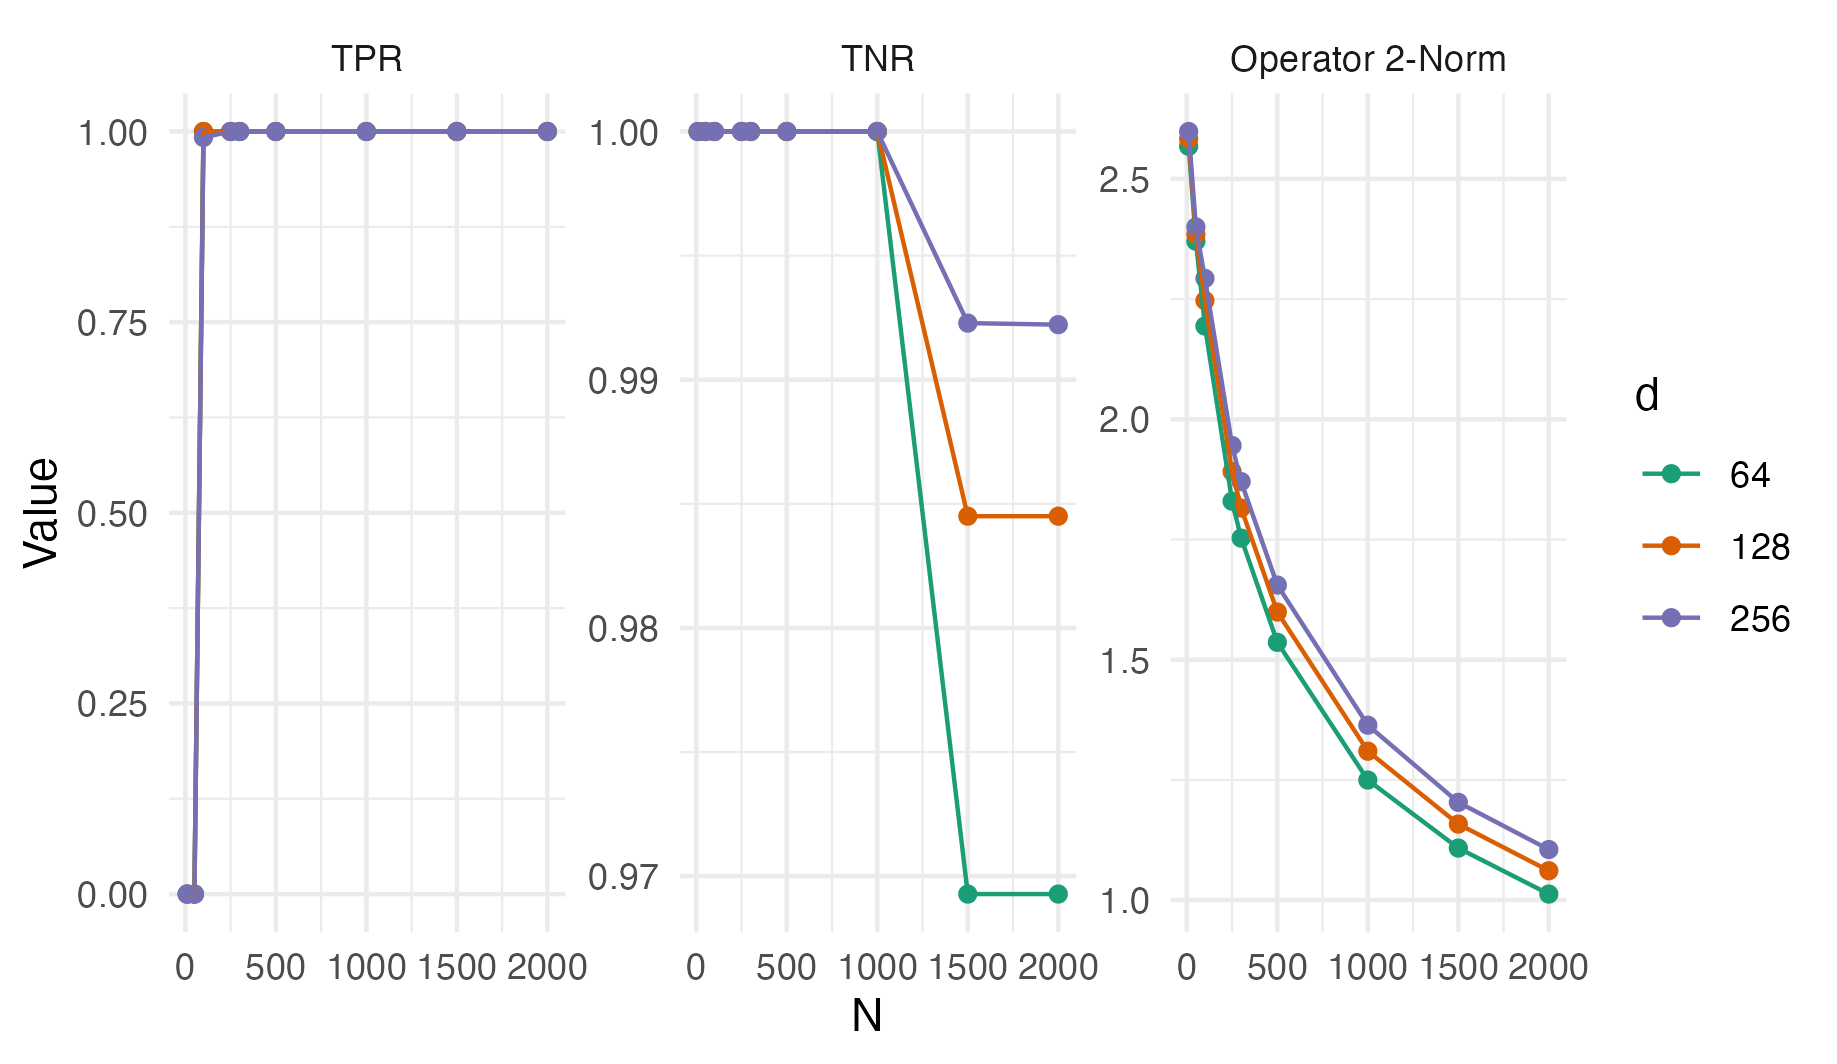
\includegraphics[scale=0.65]{glasso_complete_fixN_b1.png}
        \caption{AR(1), $\rho=0.4$ adjacency structure}
    \end{figure}
\end{frame}


\begin{frame}{Simulations (GLASSO - Complete Data)}
    \begin{figure}
        \centering 
        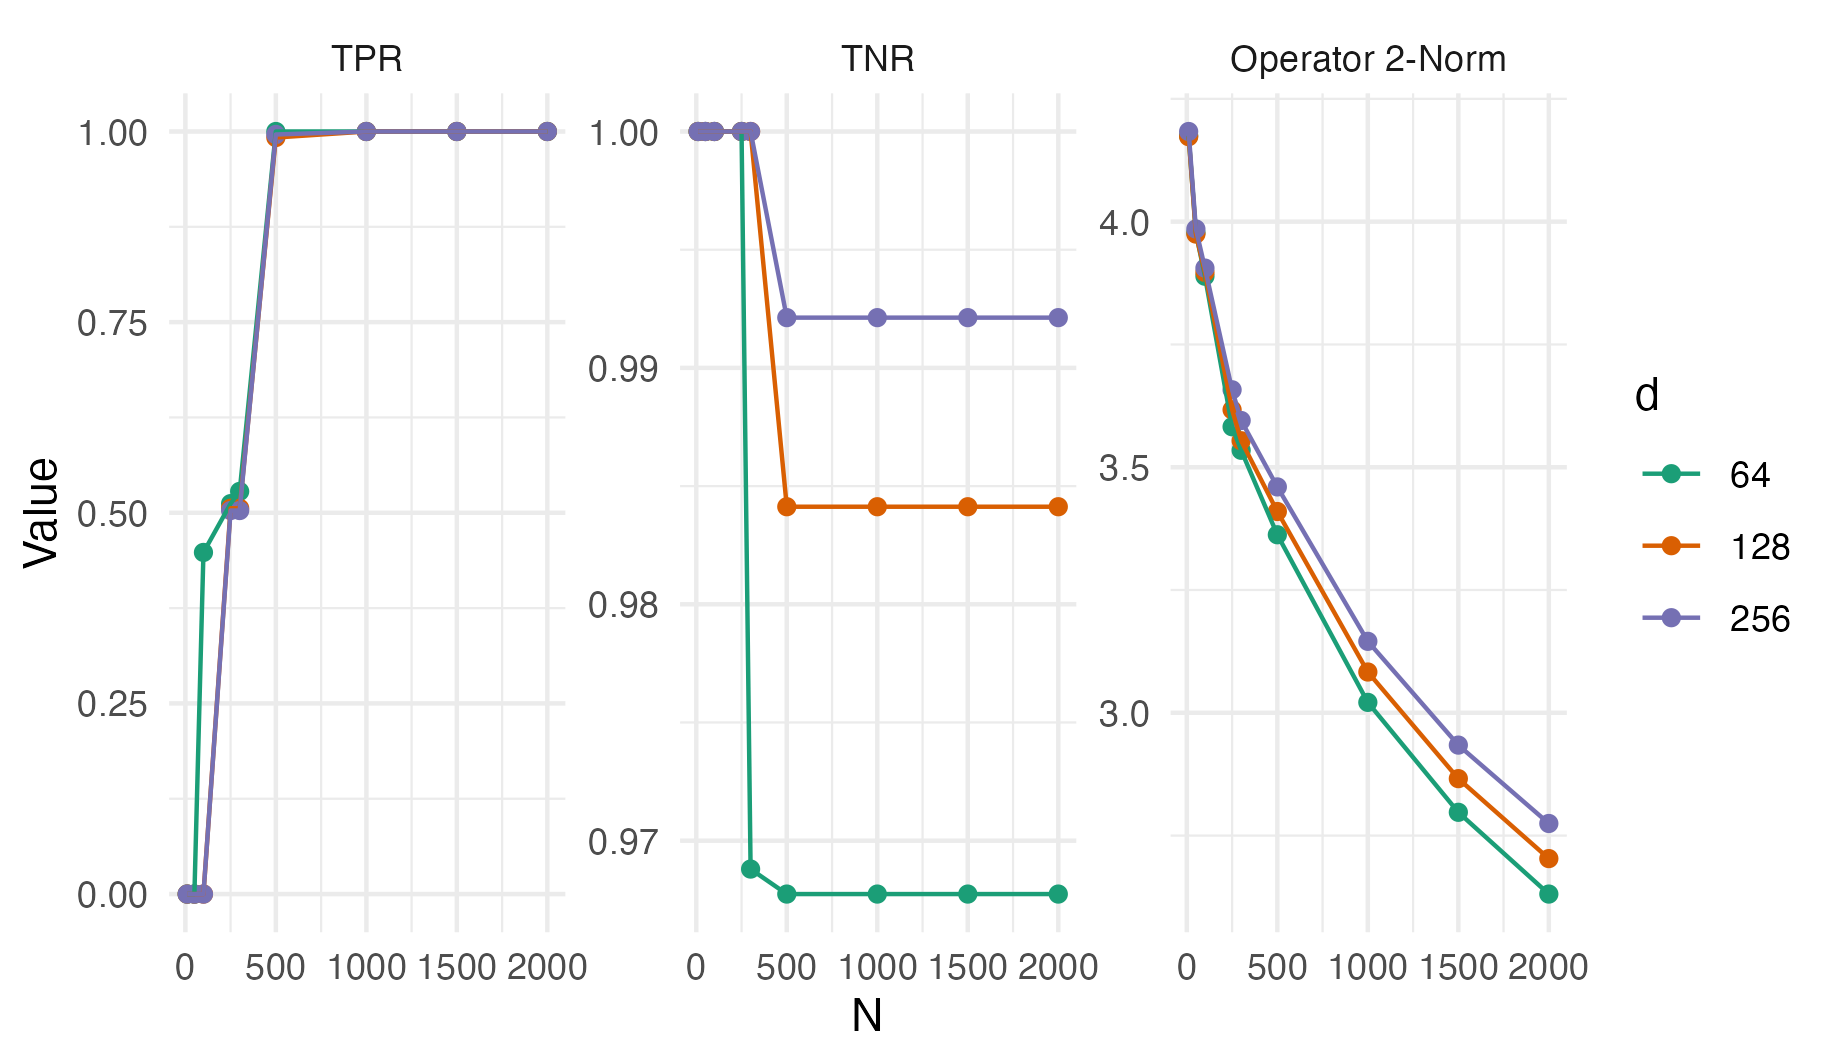
\includegraphics[scale=0.65]{glasso_complete_fixN_b2.png}
        \caption{AR(2), $\rho=0.4$ adjacency structure}
    \end{figure}
\end{frame}


\begin{frame}{Simulations (GLASSO - Complete Data)}
    \begin{figure}
        \centering 
        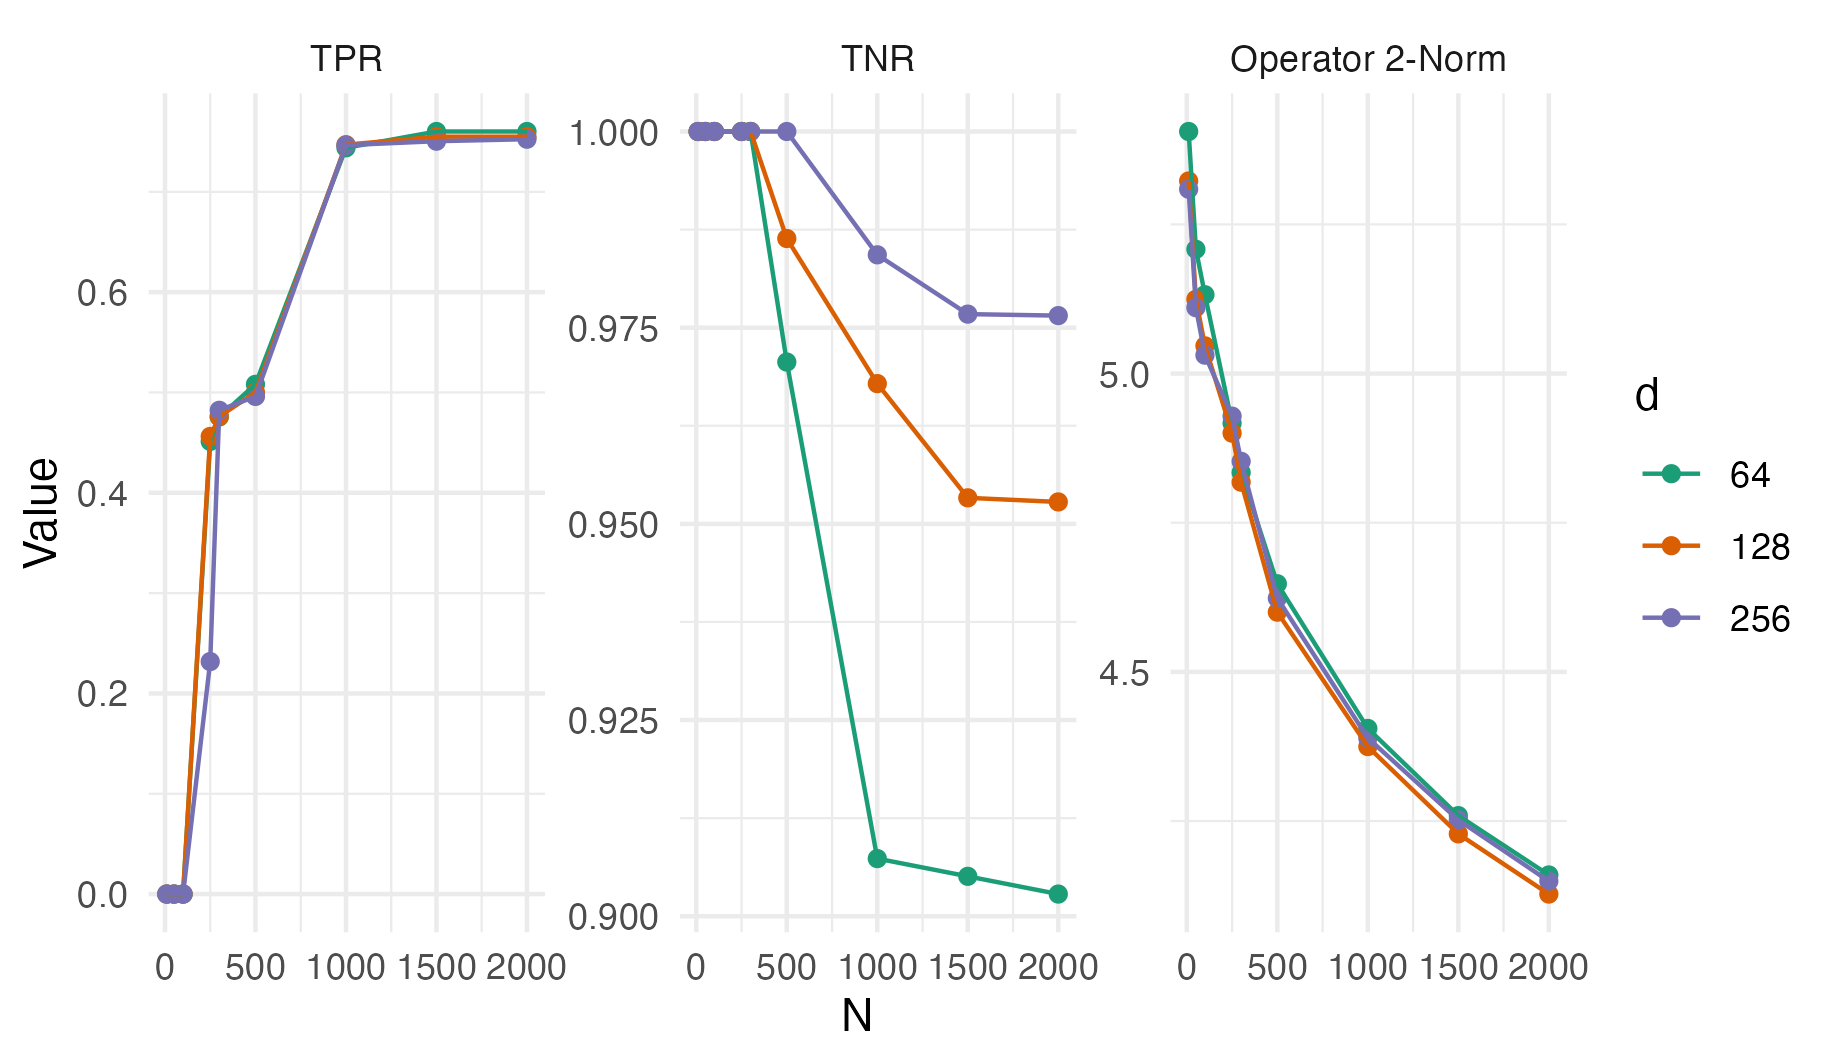
\includegraphics[scale=0.65]{glasso_complete_fixN_b4.png}
        \caption{AR(4), $\rho=0.4$ adjacency structure}
    \end{figure}
\end{frame}


\begin{frame}{Simulations (GLASSO - Complete Data)}
    \begin{figure}
        \centering 
        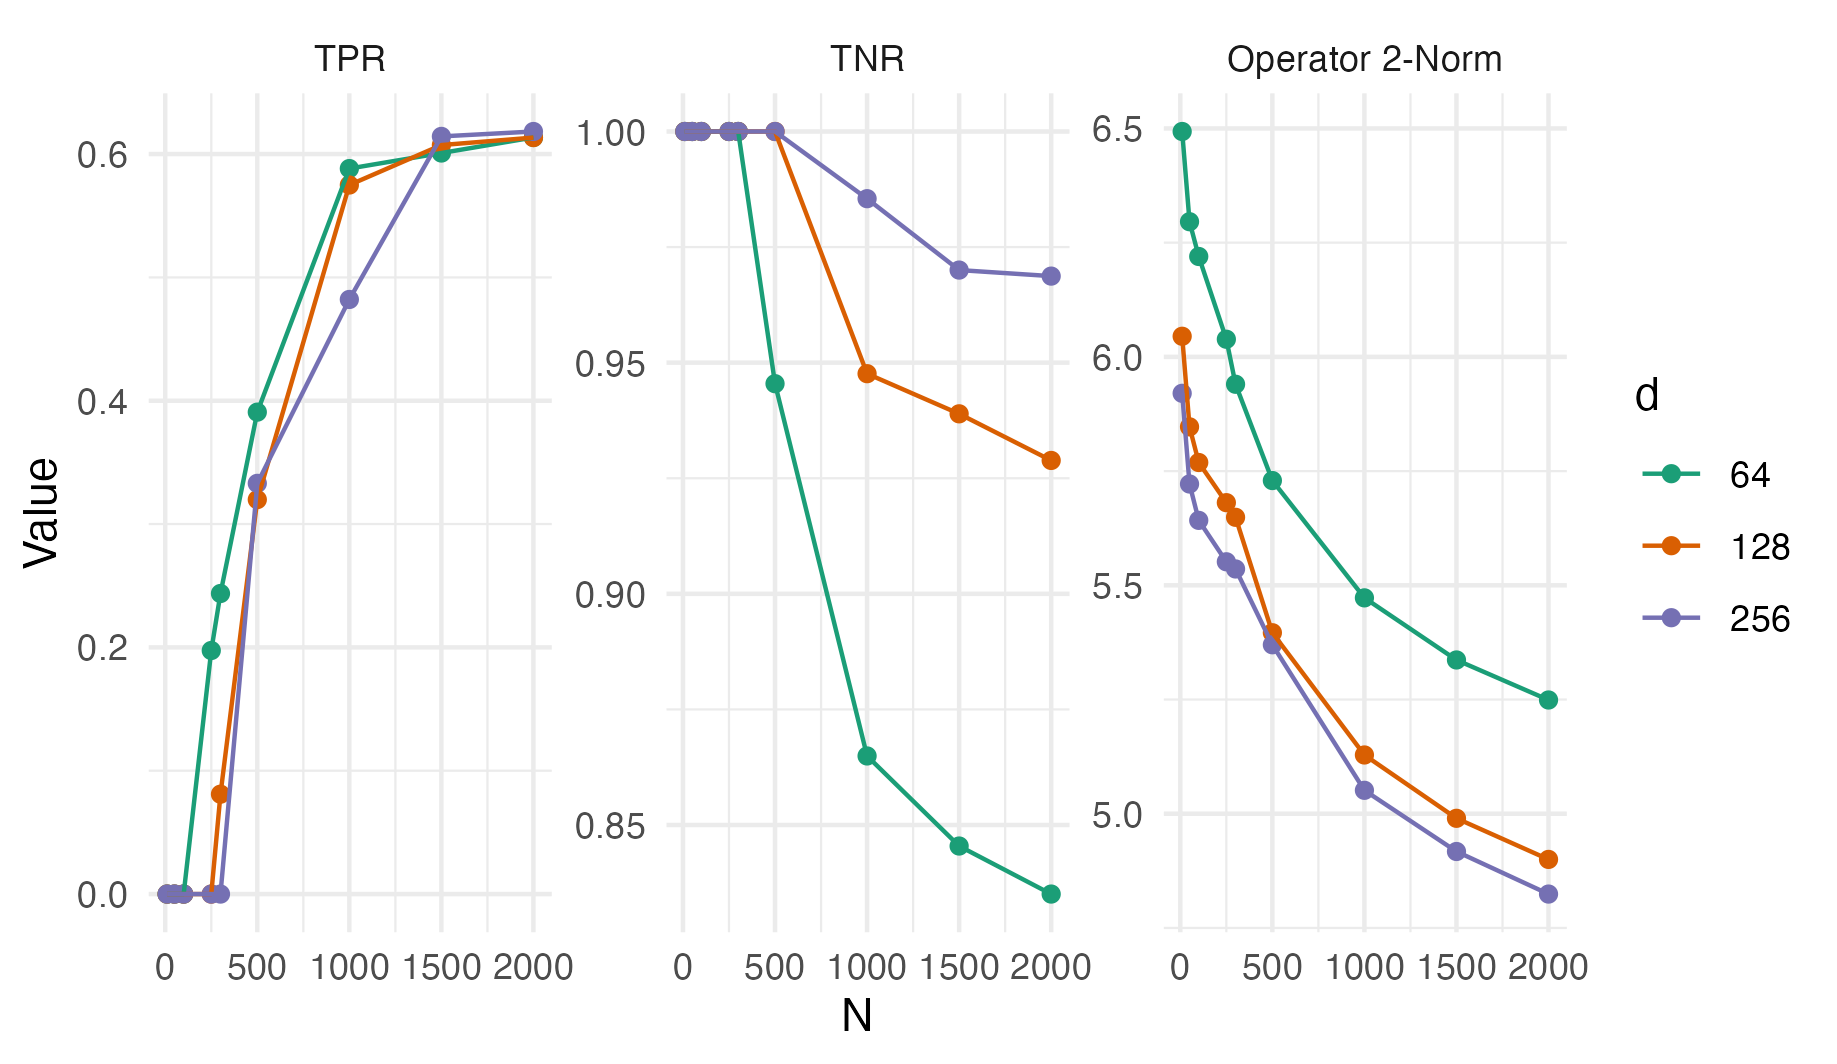
\includegraphics[scale=0.65]{glasso_complete_fixN_b8.png}
        \caption{AR(8), $\rho=0.4$ adjacency structure}
    \end{figure}
\end{frame}



\begin{frame}{Simulations (Neighborhood Selection - Complete Data)}
    \begin{figure}
        \centering 
        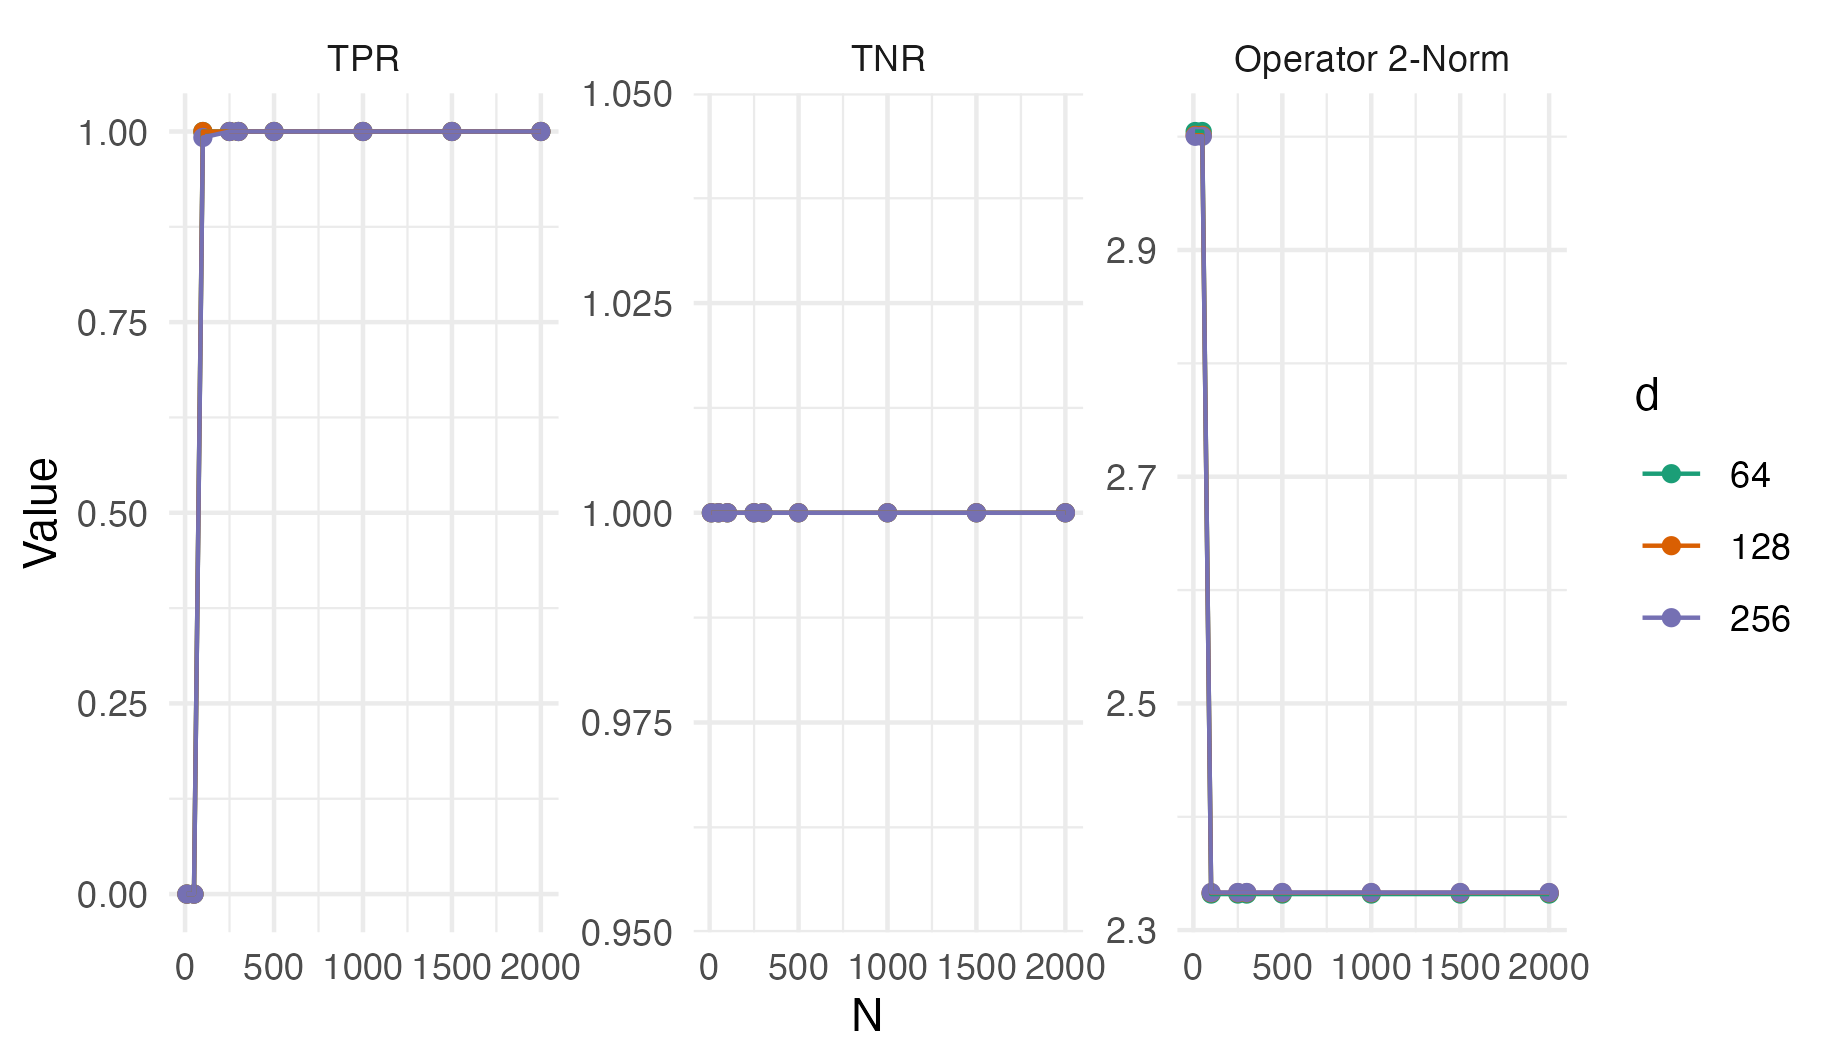
\includegraphics[scale=0.65]{glasso_complete_fixN_b1mb.png}
        \caption{AR(1), $\rho=0.4$ adjacency structure}
    \end{figure}
\end{frame}


\begin{frame}{Simulations (Neighborhood Selection - Complete Data)}
    \begin{figure}
        \centering 
        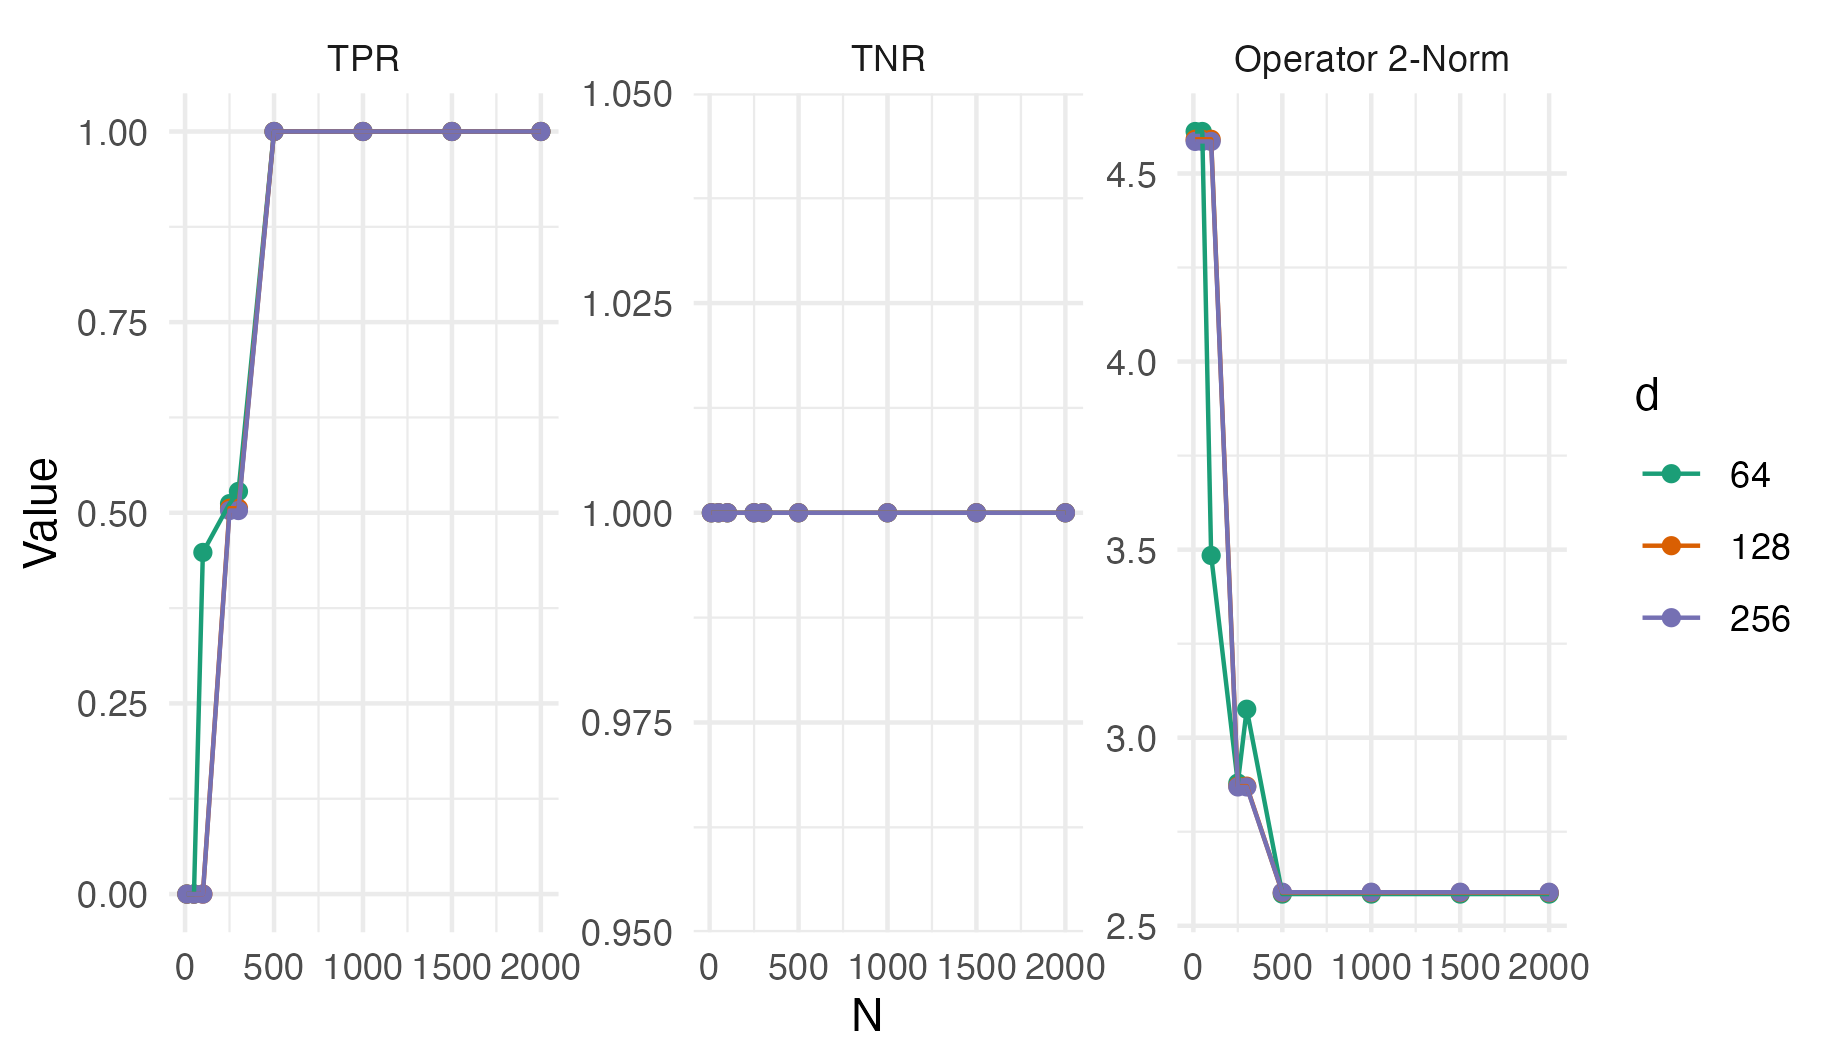
\includegraphics[scale=0.65]{glasso_complete_fixN_b2mb.png}
        \caption{AR(2), $\rho=0.4$ adjacency structure}
    \end{figure}
\end{frame}


\begin{frame}{Simulations (Neighborhood Selection - Complete Data)}
    \begin{figure}
        \centering 
        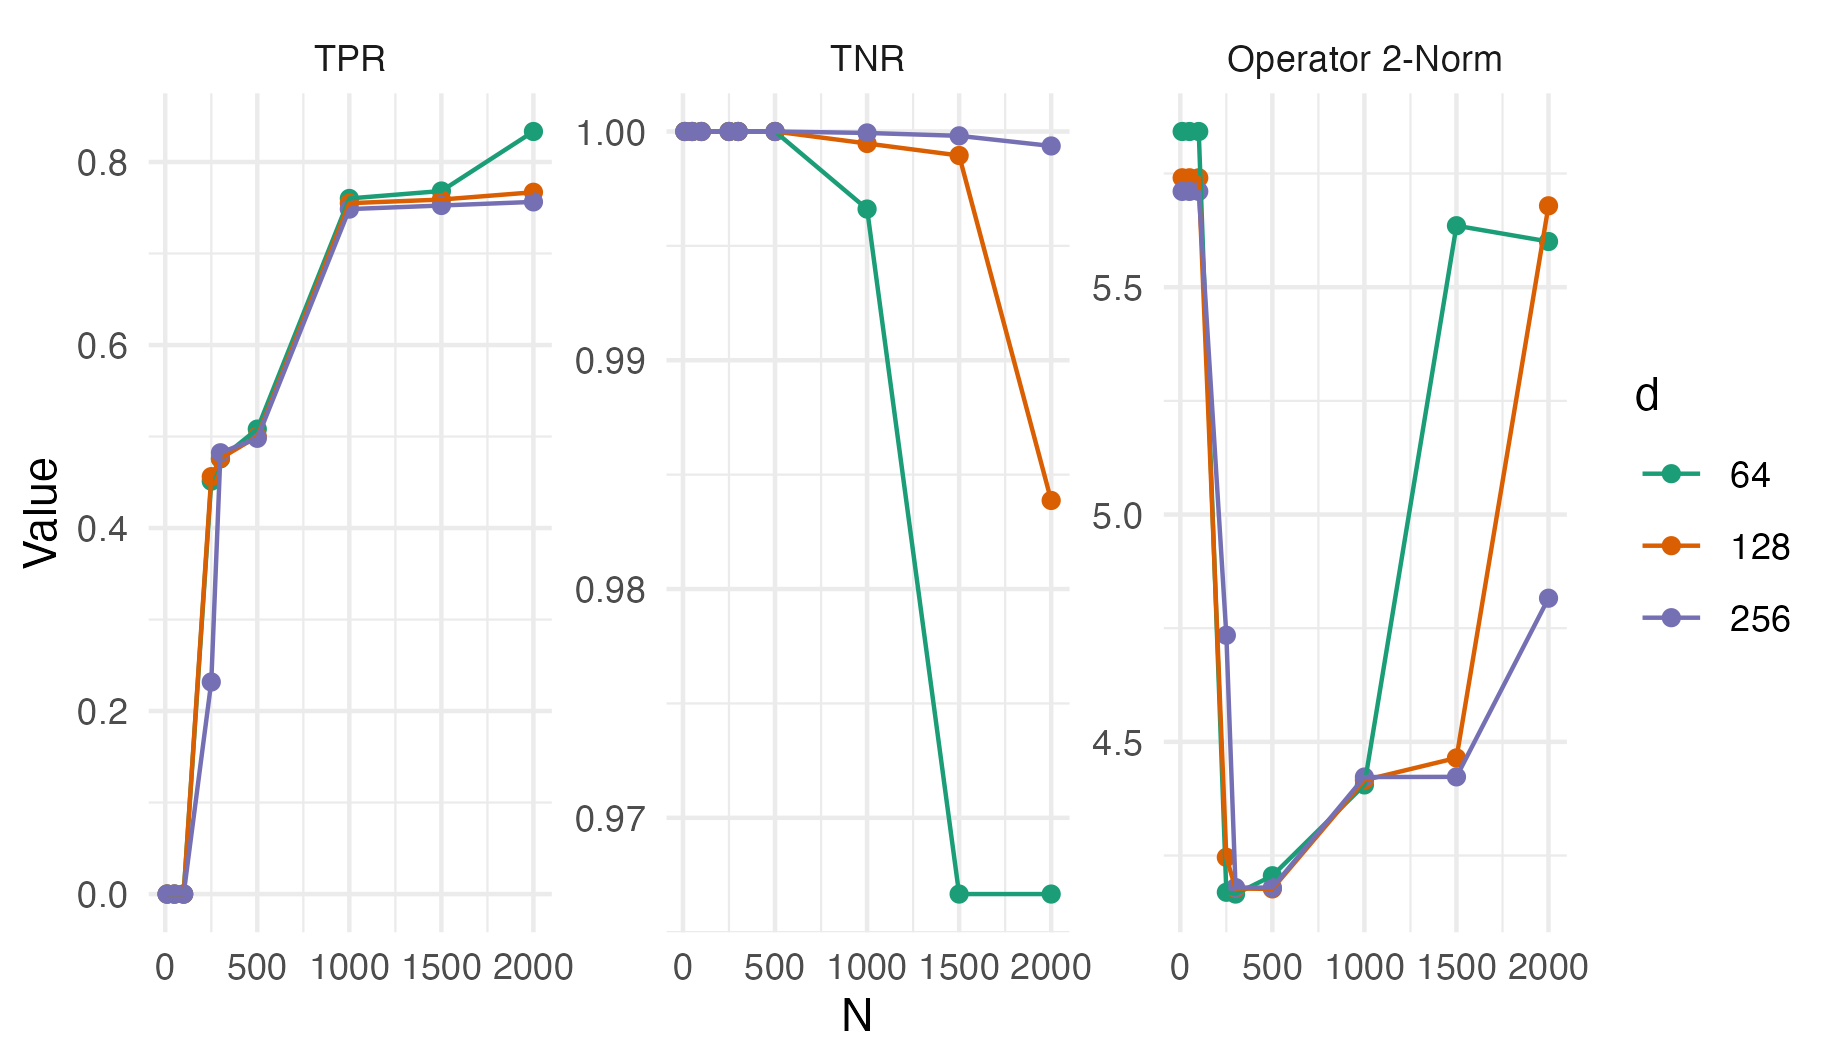
\includegraphics[scale=0.65]{glasso_complete_fixN_b4mb.png}
        \caption{AR(4), $\rho=0.4$ adjacency structure}
    \end{figure}
\end{frame}


\begin{frame}{Simulations (Neighborhood Selection - Complete Data)}
    \begin{figure}
        \centering 
        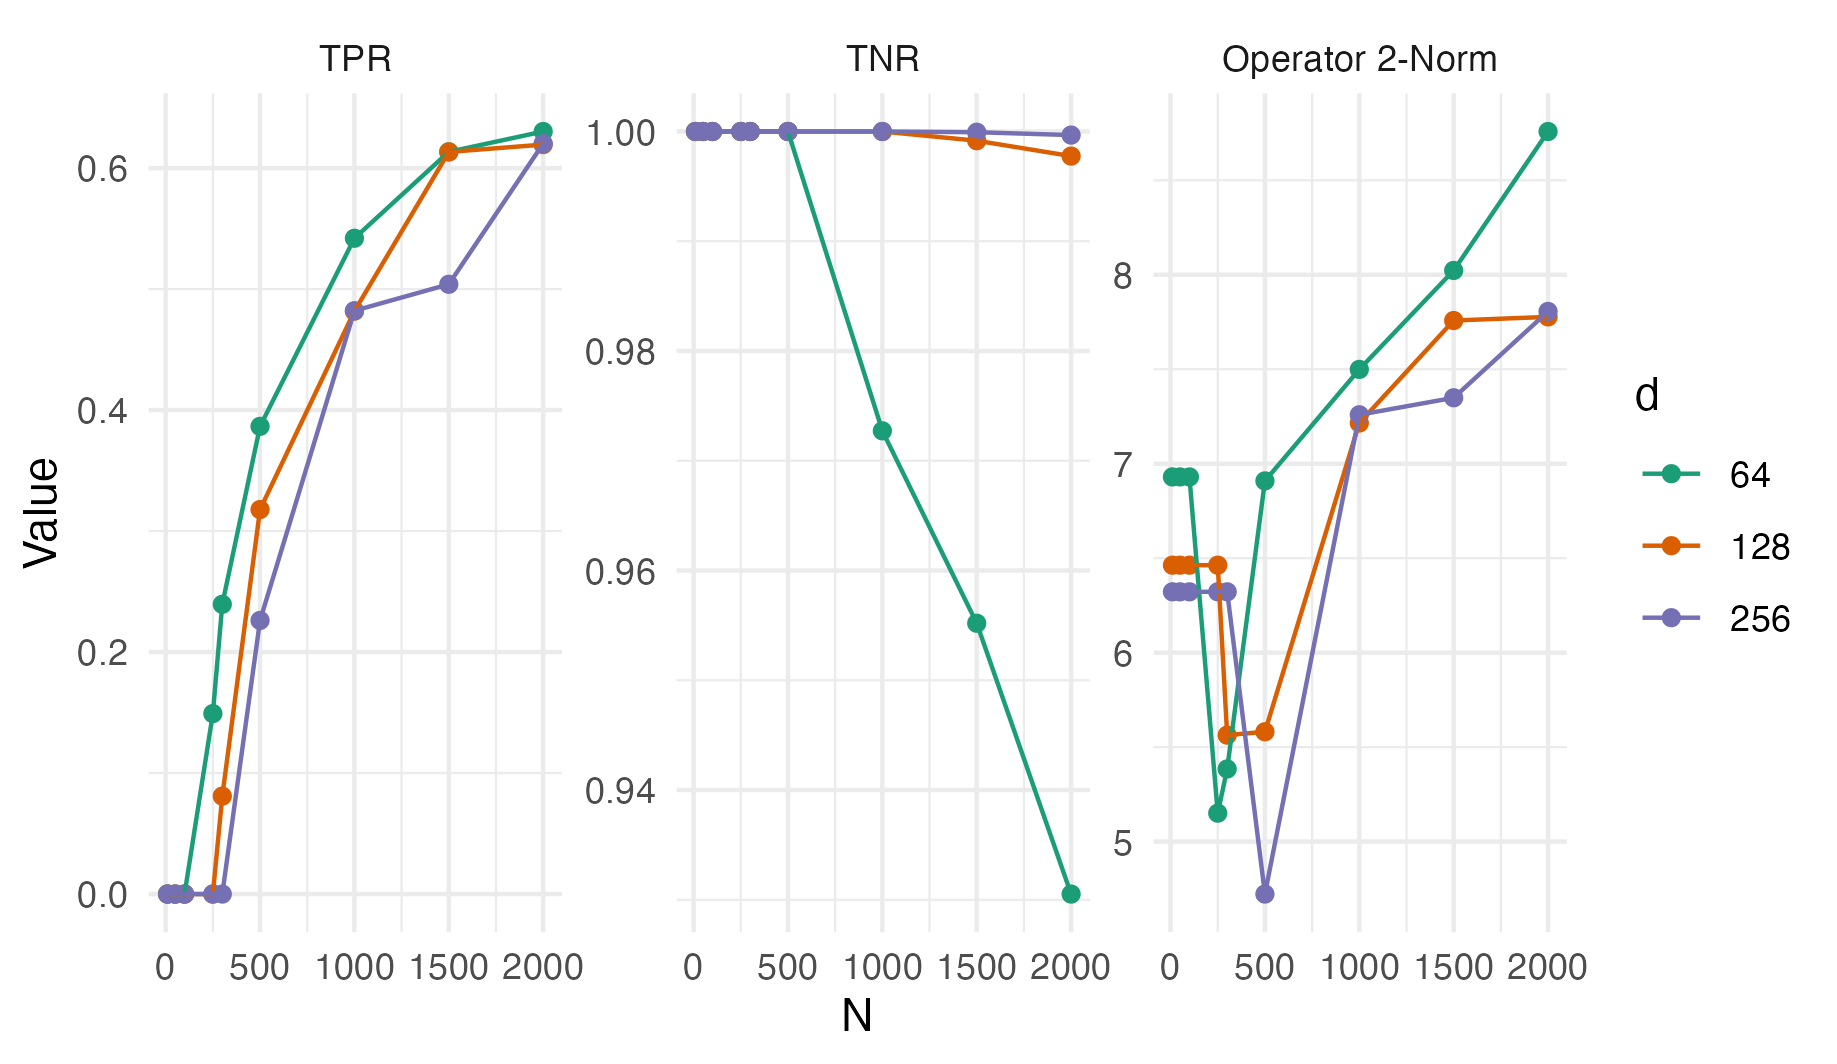
\includegraphics[scale=0.65]{glasso_complete_fixN_b8mb.png}
        \caption{AR(8), $\rho=0.4$ adjacency structure}
    \end{figure}
\end{frame}



\subsection{Further Notes}

\begin{frame}{Further Notes}
\begin{itemize}\setlength\itemsep{5mm}
%    \item Neighborhood Selection maximizes $d$ conditional likelihoods
%    \item GLasso maximizes an $\ell_1$ penalized, joint (Gaussian) likelihood
    \item Neighborhood selection (slightly) seems to outperform GLasso in edge-selection, more notably in our less-sparse settings\footnote{These results are also slightly altered by choice of $\rho$, our value $\rho=0.3$ was chosen arbitrarily and kept constant only for brevity}
    \item GLasso "better approximate" $\boldsymbol\Theta$ with asymptotic guarantees not provided by neighborhood selection
    \item Error scaling more vulnerable to $D_{max}$ than $d$-dimensionalty of random vector 
    \item Omitted results for random Erd\"os R\'enyi graphs yield similar results, conclusions 
%    \item (Highly non-trivial) extensions beyond Gaussianity exist:
%    \begin{itemize}
%        \item Heterogenous graphs (specifically mixture of Gaussian, Exponential, Poisson, Binomial nodes ) \cite{chen_selection_2015} 
 %       \item Non-parametric extensions \cite{dong_nonparametric_2022}
 %   \end{itemize}
\end{itemize}    
\end{frame}


\section{Estimation with Missingness}

\begin{frame}{Motivation}
    \begin{itemize}
        \item Methods above largely assume complete data\footnote{In the Gaussian setting, hidden/unobserved nodes or missingness can be mean-imputed, but this is fairly n\"aive/ad-hoc procedure}
        \item Networks change, measurement availability (and quality) varies
        \item Measurement is also often differential between nodes 
    \end{itemize}
    \textcolor{red}{Visualization here}
\end{frame}

\begin{frame}{Na\"ive Methods with Missingness}
    \textcolor{red}{Results with nhood, GLasso in grahpicswith missingness}
\end{frame}

\subsection{General Methods}

\begin{frame}{Graphical Methods for Missingness}
\end{frame}

\subsection{{\it Erose} Data and GI-JOE}



\begin{frame}{{\it Erose} Data}
    \begin{itemize}
        \item {\it Erose} data is a term coined by Zheng, Allen (2023) for data with irregular availability \cite{zheng_gi-joe_2023}
        \begin{itemize}
            \item Leads to "drastically different" sample size for a small subset of nodes 
            \item Erose data almost certainly violate MAR/MCAR assumptions of existing methods 
            \item Motivated by neuroscience but with applications in genetic expression data, 
        \end{itemize}
    \end{itemize} 
\end{frame}


\begin{frame}{GI-JOE for Erose Data}
\end{frame}


\section*{Conclusion}

\begin{frame}{Graphs, how and why (revisited)?}
    \centering
    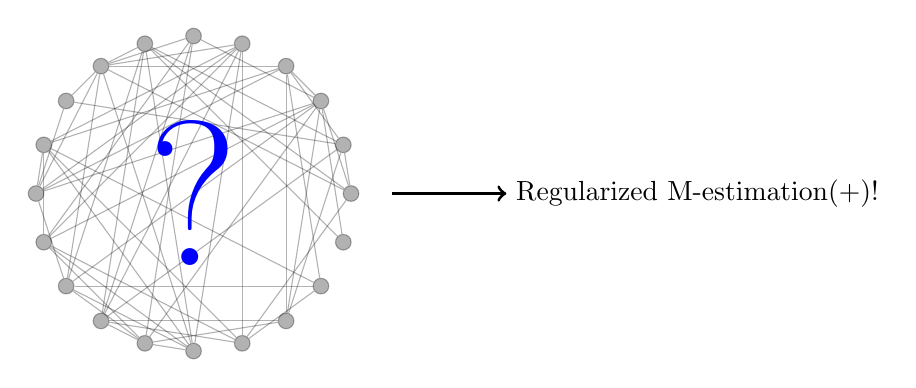
\begin{tikzpicture}[opacity=0.3]
        \foreach \i in {1,...,20} {
            \node[circle, draw, fill=black, inner sep=2pt] (node\i) at ({360/20 * (\i - 1)}:2) {};
          }
        
          \foreach \i in {1,...,19} {
            \foreach \j in {\i,...,20} {
              \ifnum\i<\j
                \pgfmathparse{rnd}
                \ifdim\pgfmathresult pt<0.3pt
                  \draw (node\i) -- (node\j);
                \fi
              \fi
            }
          }
    \node[blue, scale=3, opacity=1] (Q) at (0,0) {\Huge ?}; % Add a large question mark in the center
    \node (inv) at (2.4, 0) {};
    %\node[opacity=1] (NH) at (6.4, 0.5) {Neighborhood Selection (even with {\it erose} data)};
    \node[opacity=1] (M) at (6.4, 0) {Regularized M-estimation(+)!};
    %\node[opacity=1] (NH) at (6.4, -0.5) {Conditional GLasso models};
    \draw[->, opacity=1, line width=0.4mm] (inv) edge (M);
    \end{tikzpicture}
\end{frame}


\begin{frame}{Conclusion}
    \begin{itemize}
        \item Graphs are a powerful representation of your multivariate data (intuitively and algorithmically)
        \item Useful, theoretical extensions may follow more immediately under the graphical model formalism 
        \item These extensions tend\footnote{Under a high-dimensiona/assumed-sparsity regime} to distill to regularized M-estimation problems, an area with great theoretical contributions and guarantees
        \item Extensions beyond Gaussianity substantially increase complexity 
    \end{itemize}
\end{frame}


\begin{frame}[allowframebreaks]{References}
    \begin{itemize}
    \item Some diagrams generated in conjunction with ChatGPT 3.5
    \end{itemize}
    \printbibliography 
\end{frame}


%%%%%%%%%%%%%%%%%%%%%%%%%%
%%%%%%%%%%%%%%%%%%%%%%%%%%
% Appendix 
%%%%%%%%%%%%%%%%%%%%%%%%%%
%%%%%%%%%%%%%%%%%%%%%%%%%%

\section*{Appendix}

\begin{frame}{}
\bf{\LARGE Appendix Slides}    
\end{frame}


\begin{frame}{}
    \bf{\LARGE Erd\"os R\'enyi Graph Results (Complete Data)}    
\end{frame}
    


\begin{frame}{Simulations (GLASSO - Complete Data)}
    \begin{figure}
        \centering 
        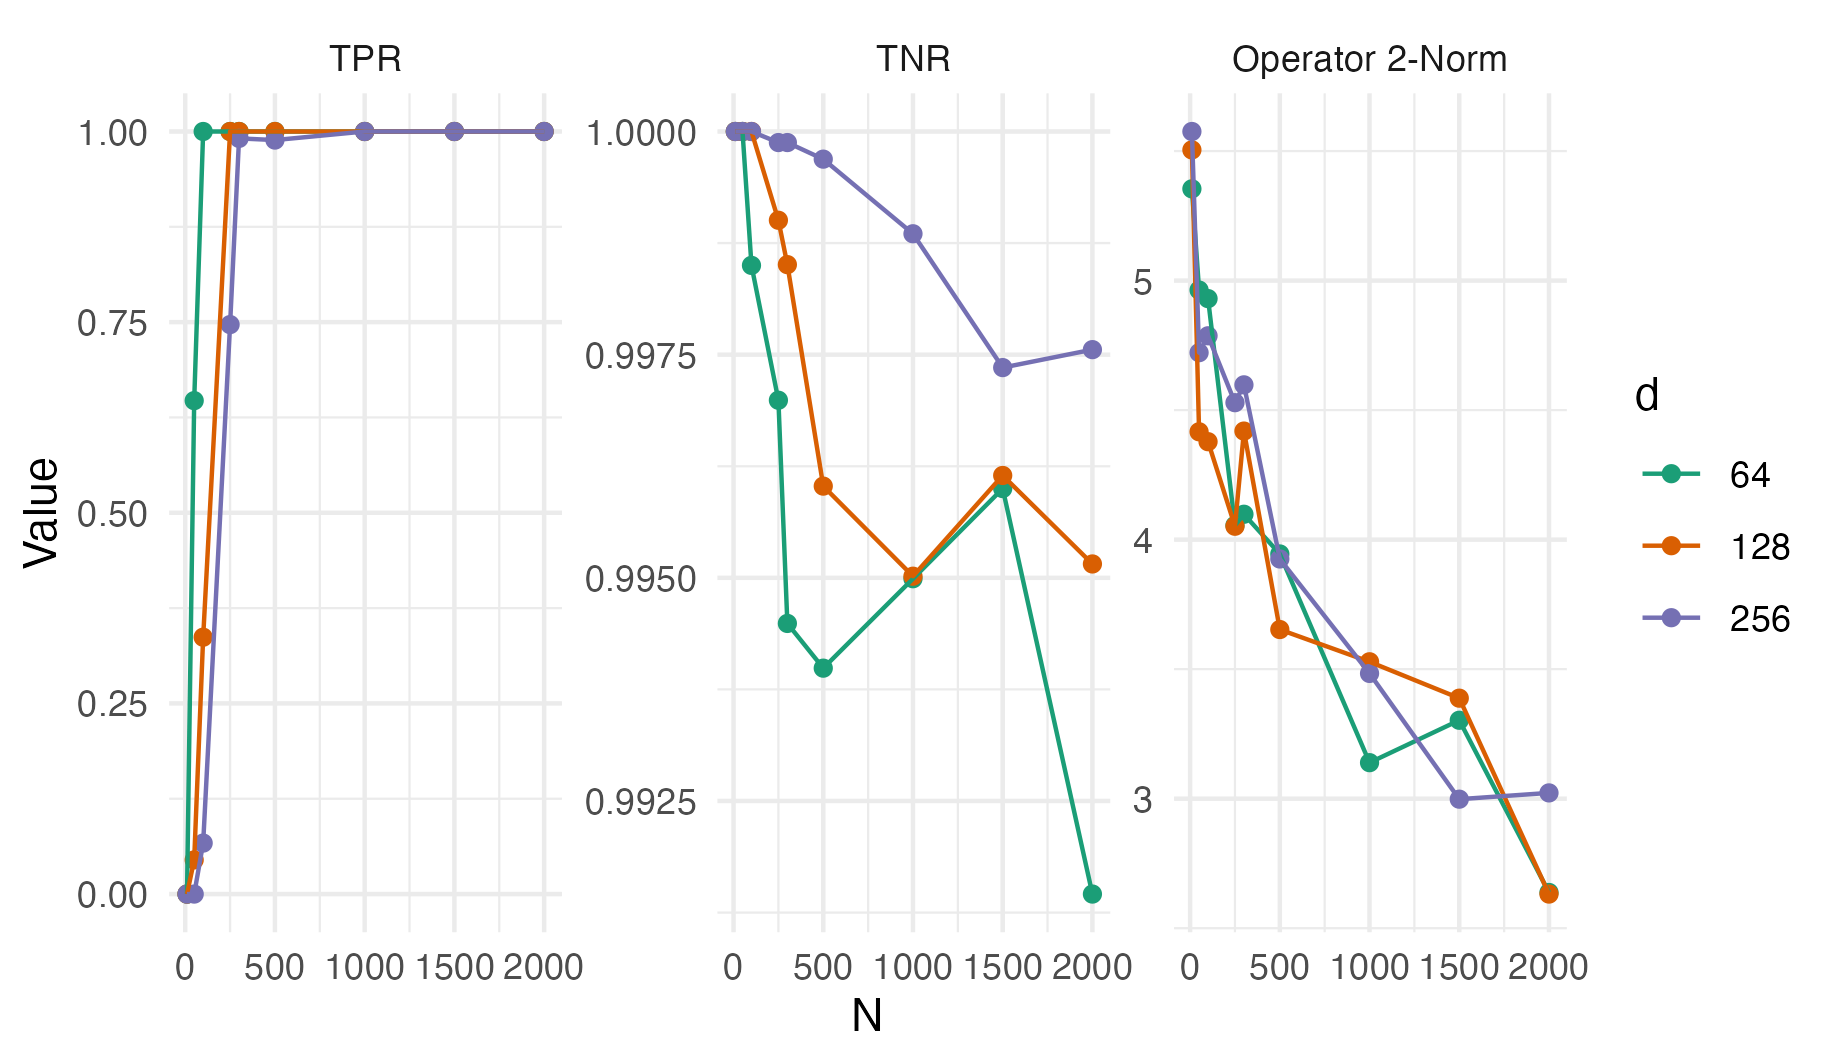
\includegraphics[scale=0.65]{glasso_complete_ER_FixN_01.png}
        \caption{ER(p=0.01), $\rho=0.4$ adjacency structure}
    \end{figure}
\end{frame}


\begin{frame}{Simulations (GLASSO - Complete Data)}
    \begin{figure}
        \centering 
        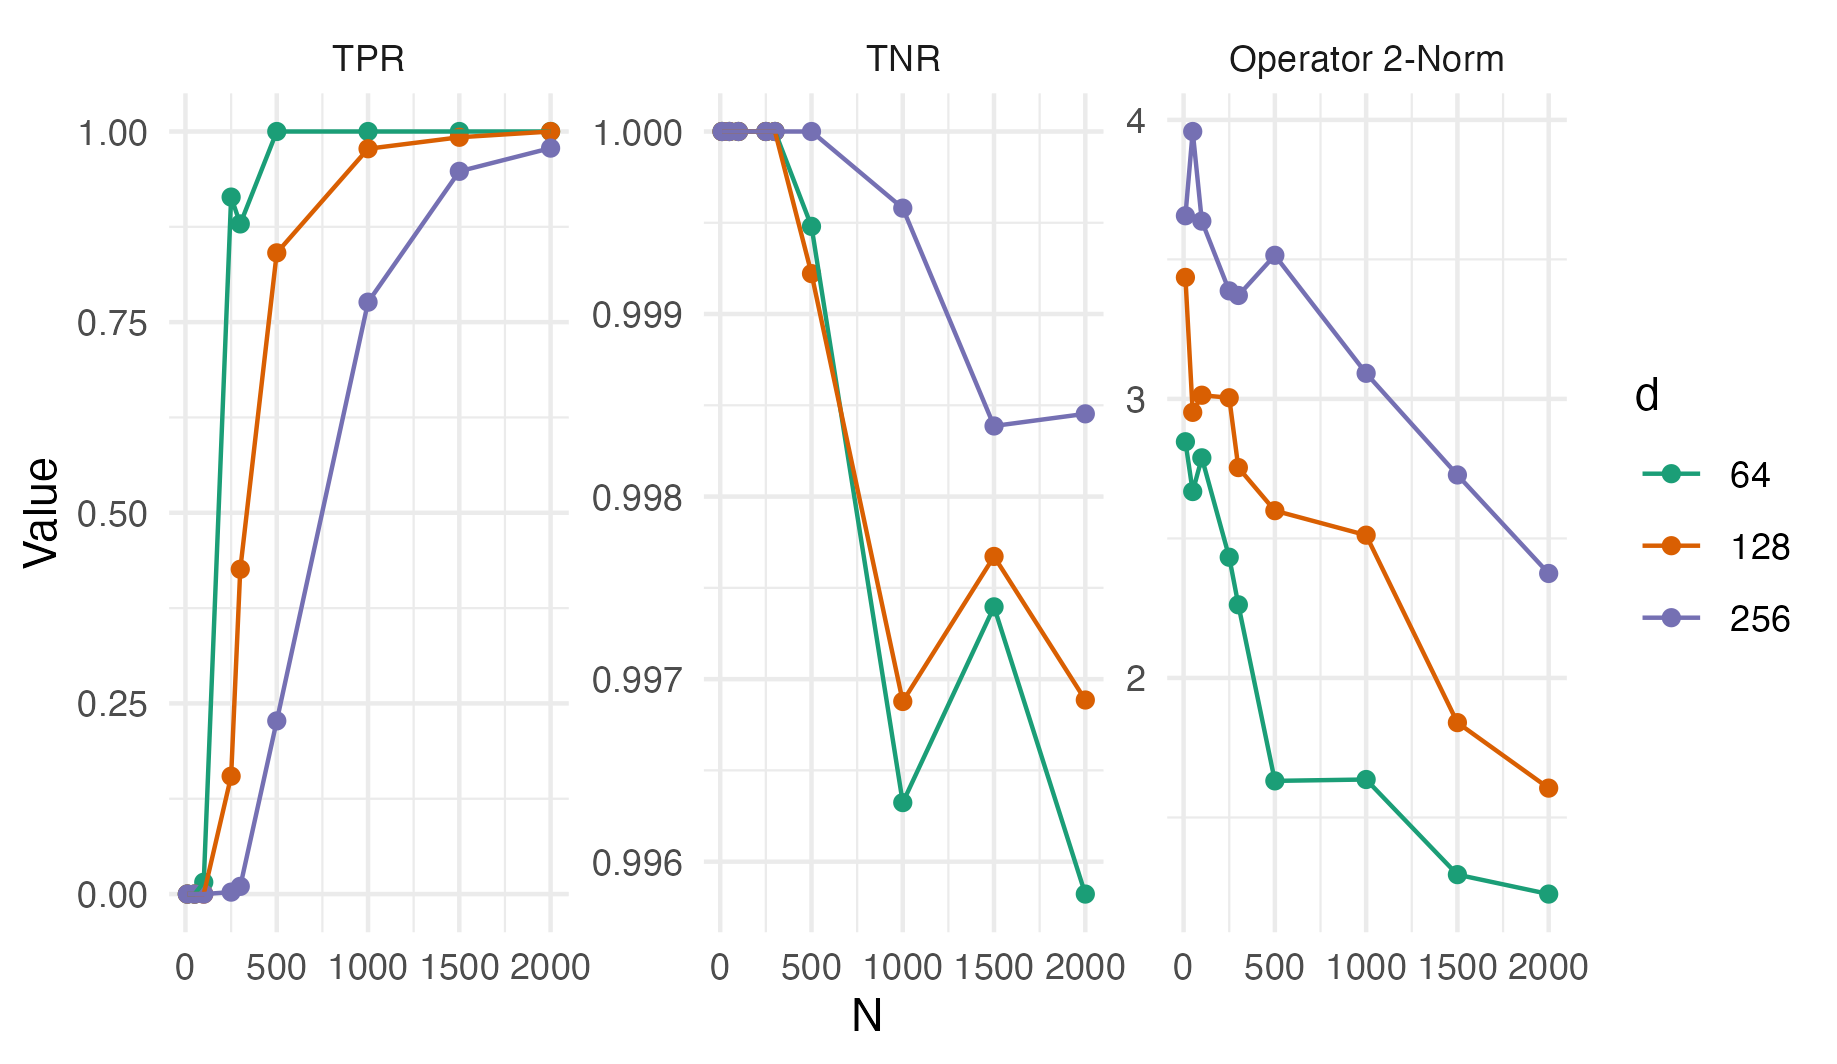
\includegraphics[scale=0.65]{glasso_complete_ER_FixN_05.png}
        \caption{ER(p=0.05), $\rho=0.4$ adjacency structure}
    \end{figure}
\end{frame}


\begin{frame}{Simulations (GLASSO - Complete Data)}
    \begin{figure}
        \centering 
        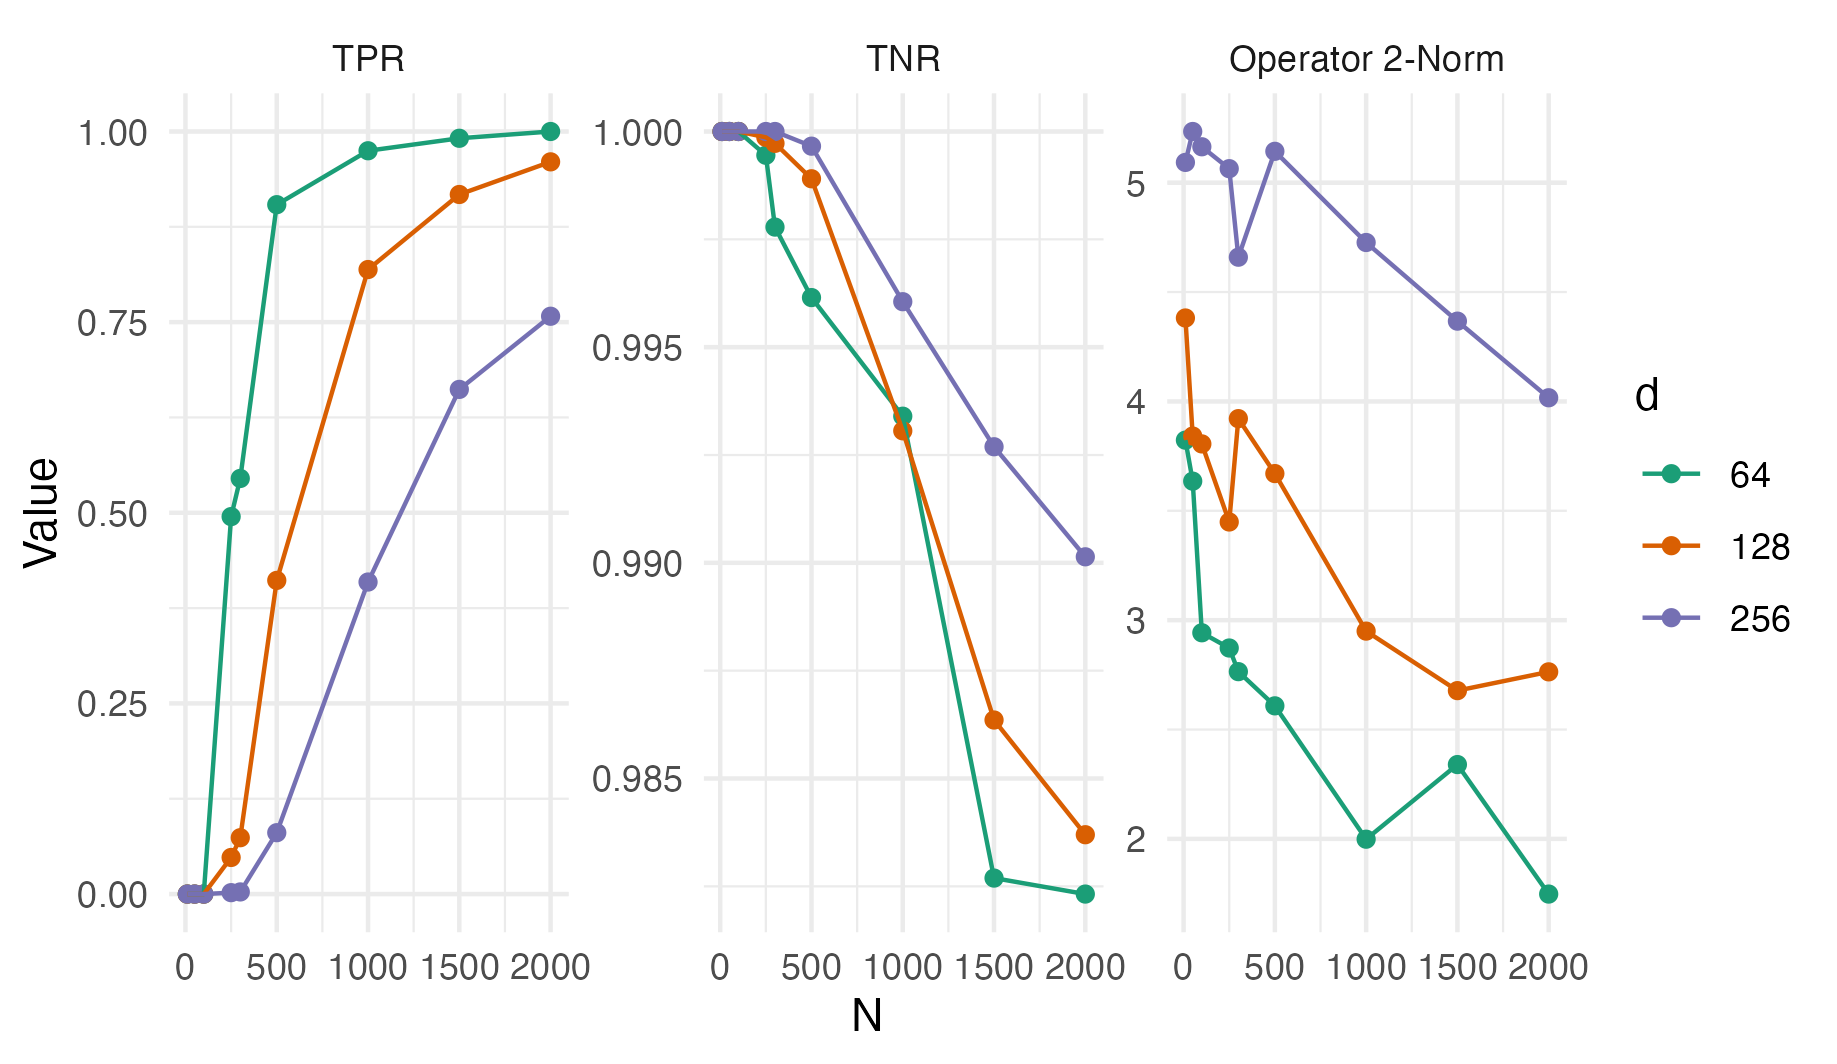
\includegraphics[scale=0.65]{glasso_complete_ER_FixN_1.png}
        \caption{ER(p=0.1), $\rho=0.4$ adjacency structure}
    \end{figure}
\end{frame}


\begin{frame}{Simulations (GLASSO - Complete Data)}
    \begin{figure}
        \centering 
        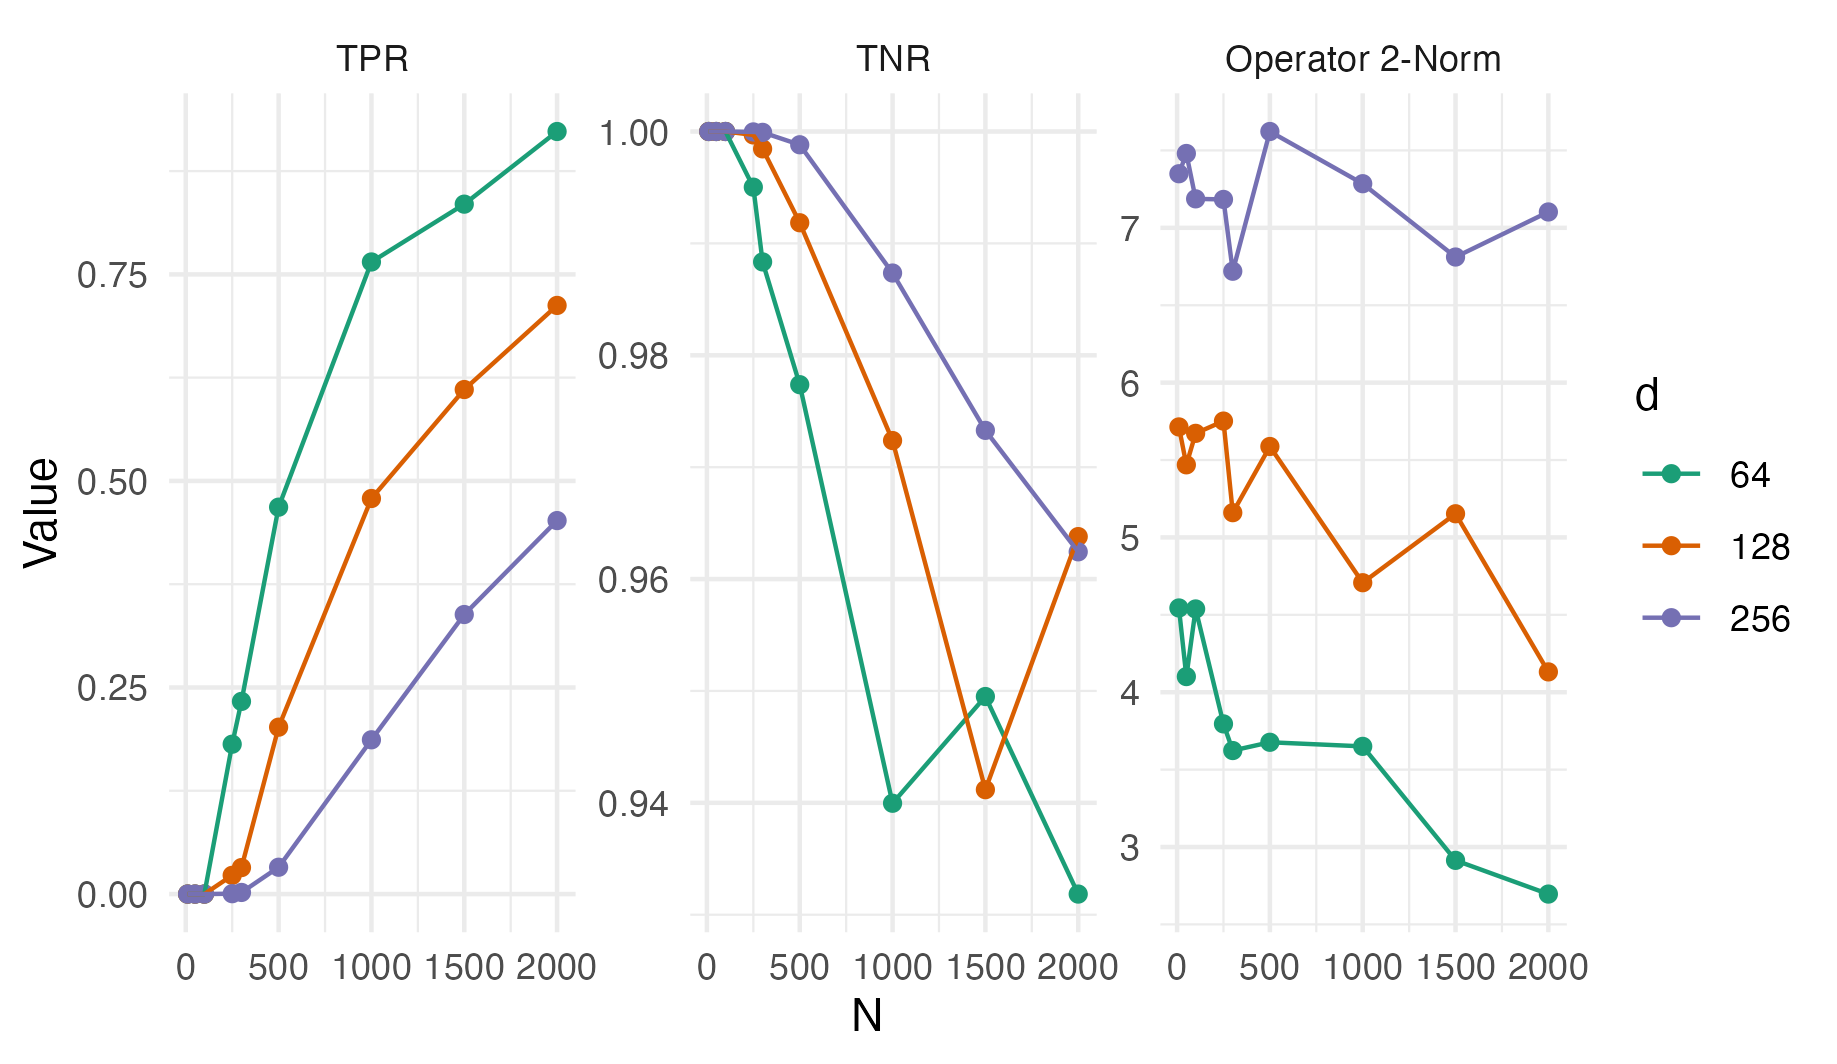
\includegraphics[scale=0.65]{glasso_complete_ER_FixN_2.png}
        \caption{ER(p=0.2), $\rho=0.4$ adjacency structure}
    \end{figure}
\end{frame}



\begin{frame}{ER-Simulations (Neighborhood Selection - Complete Data)}
    \begin{figure}
        \centering 
        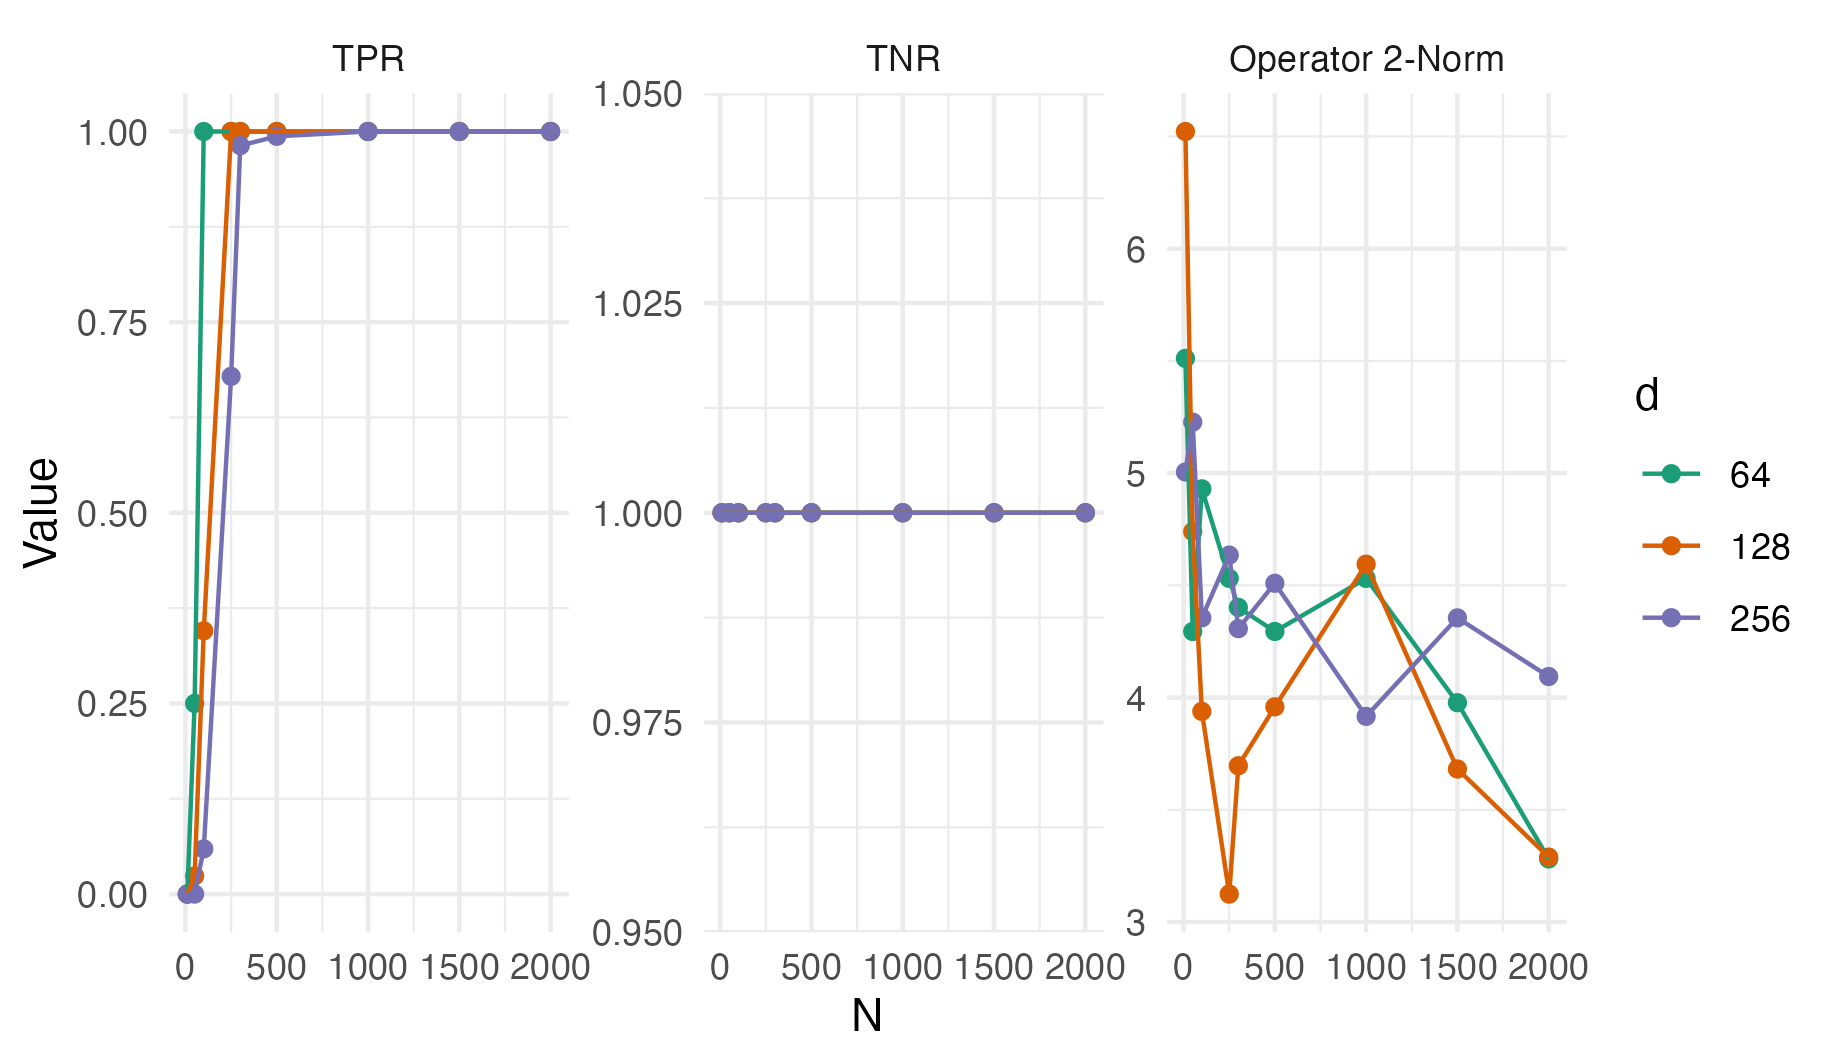
\includegraphics[scale=0.65]{glasso_complete_ERmb_FixN_01.png}
        \caption{ER(p=0.01), $\rho=0.4$ adjacency structure}
    \end{figure}
\end{frame}


\begin{frame}{ER-Simulations (Neighborhood Selection - Complete Data)}
    \begin{figure}
        \centering 
        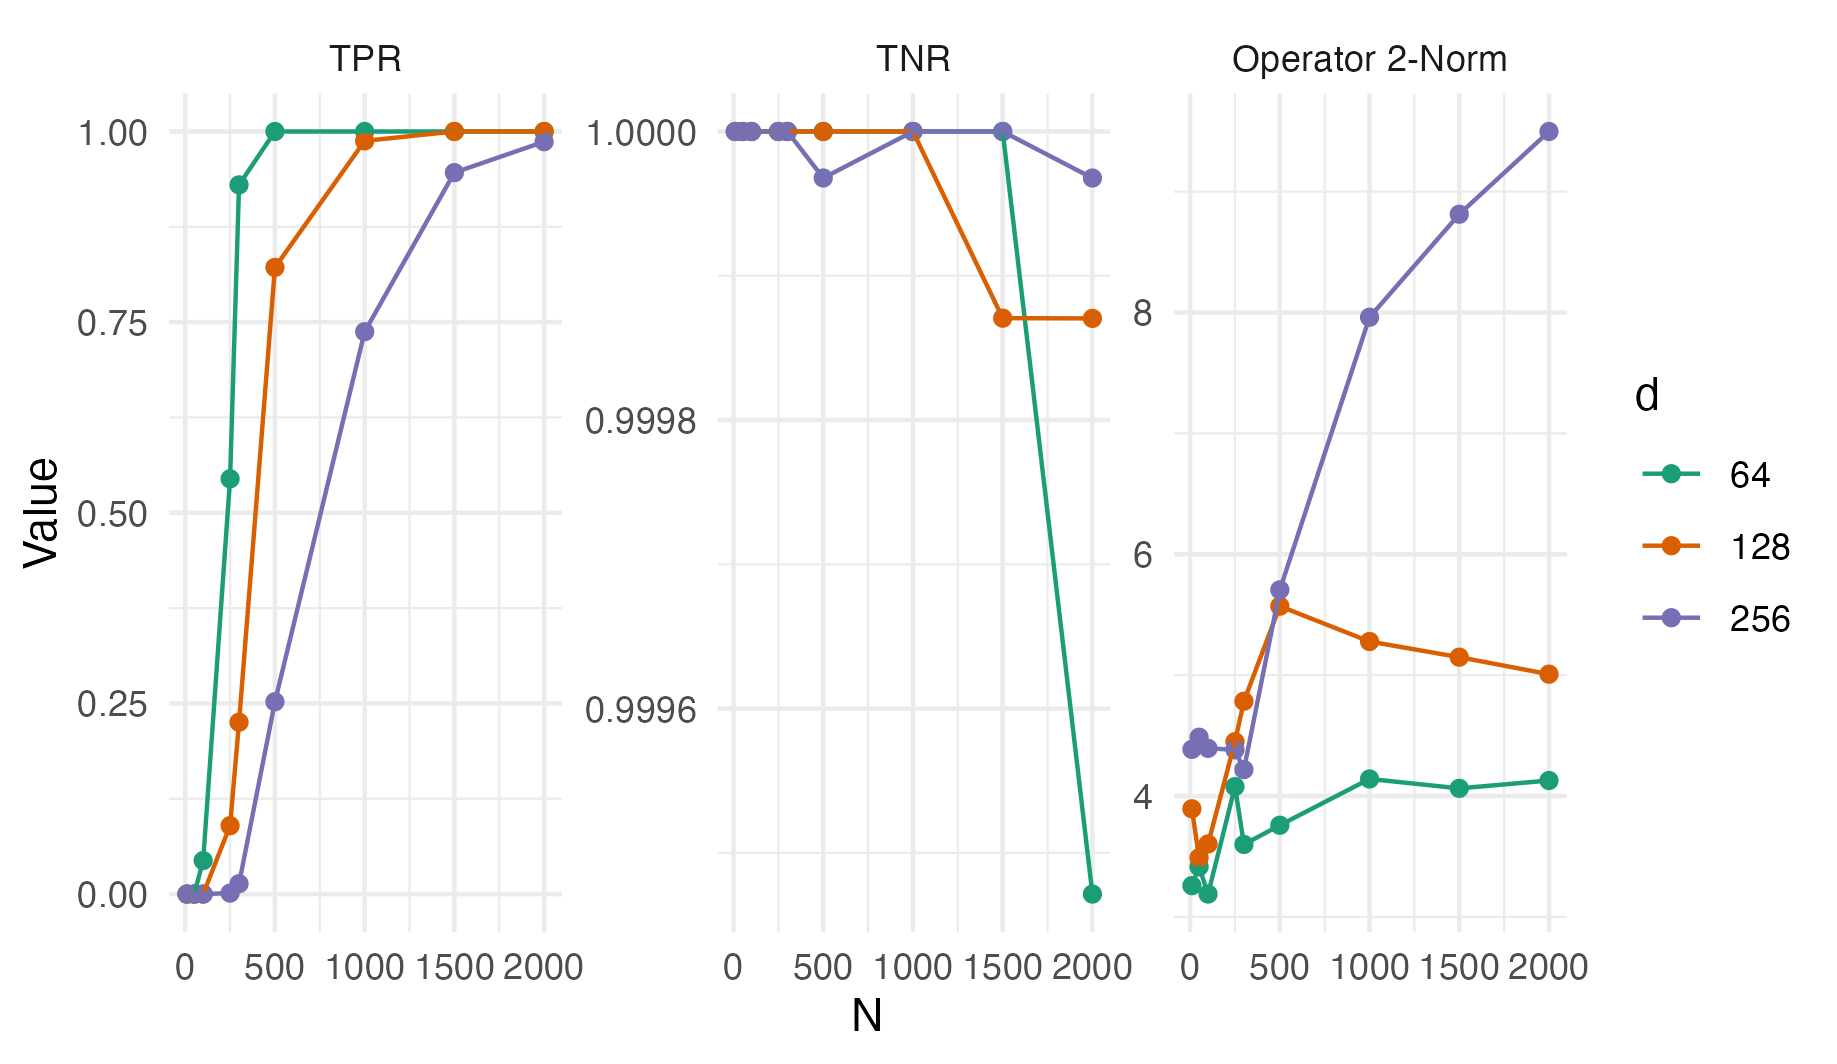
\includegraphics[scale=0.65]{glasso_complete_ERmb_FixN_05.png}
        \caption{ER(p=0.05), $\rho=0.4$ adjacency structure}
    \end{figure}
\end{frame}


\begin{frame}{ER-Simulations (Neighborhood Selection - Complete Data)}
    \begin{figure}
        \centering 
        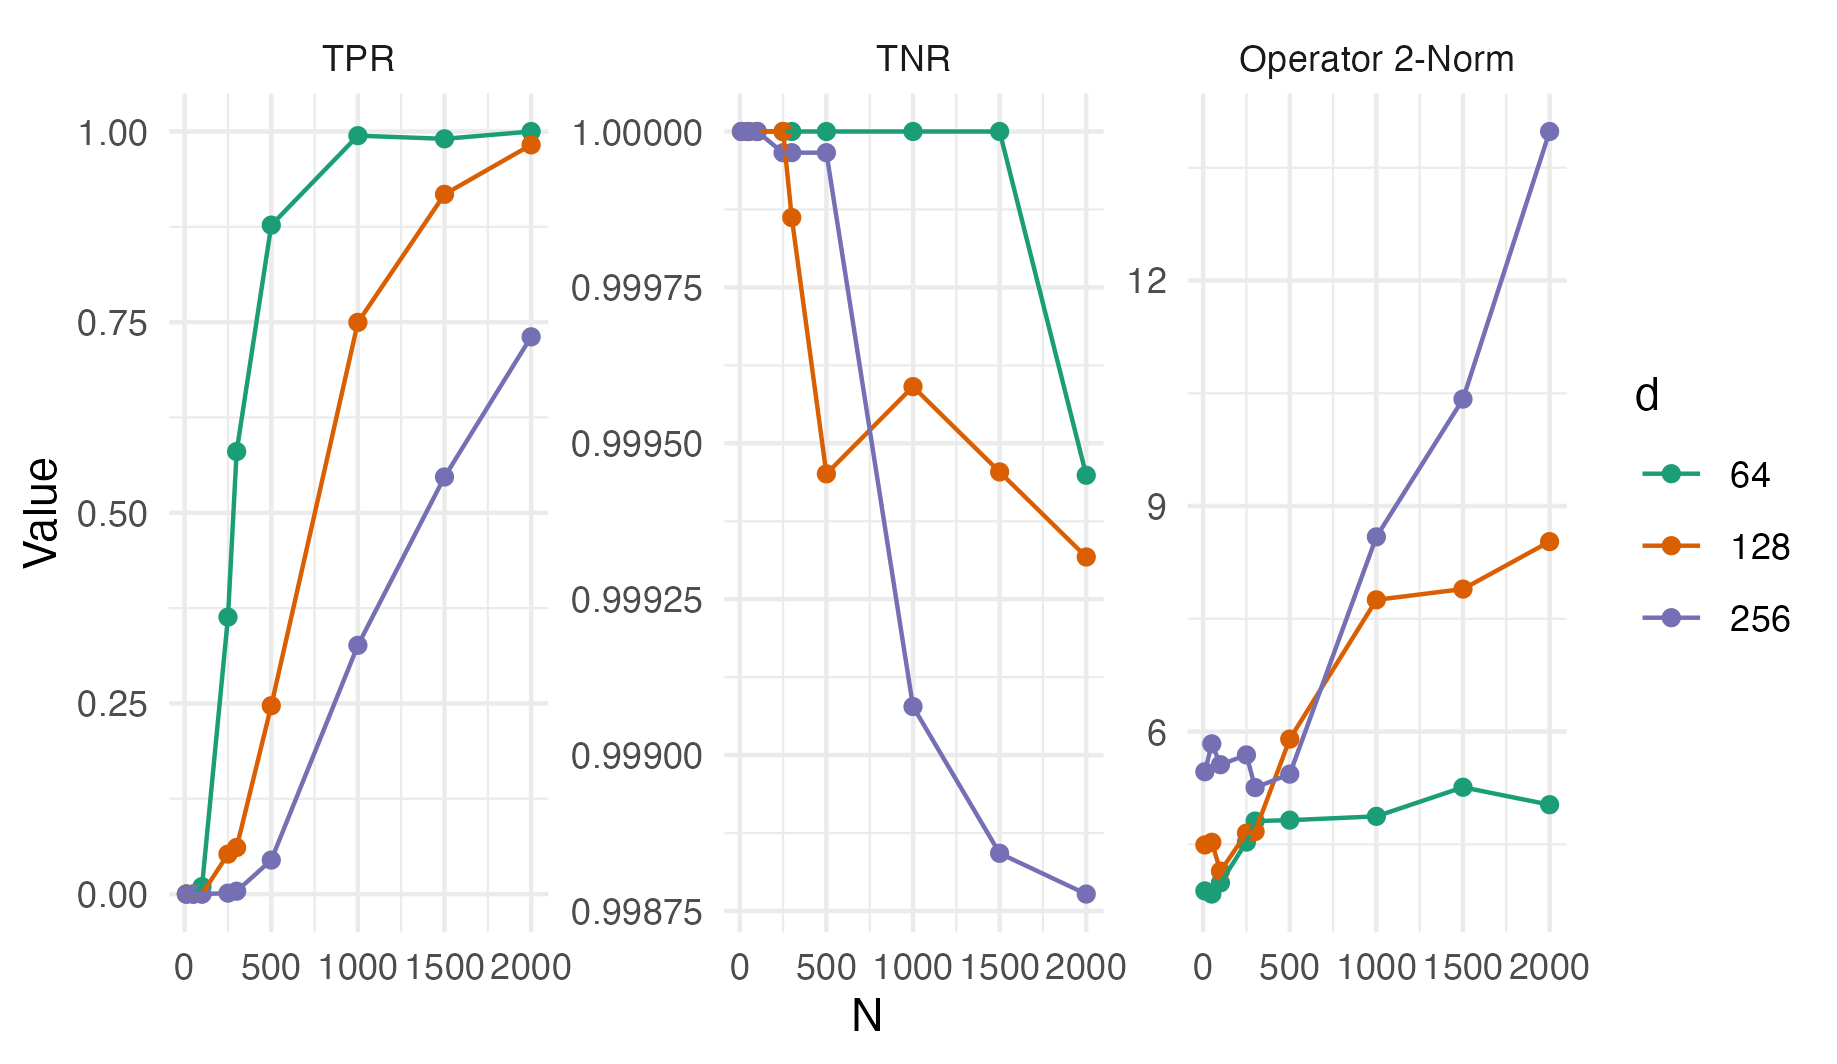
\includegraphics[scale=0.65]{glasso_complete_ERmb_FixN_1.png}
        \caption{ER(p=0.1), $\rho=0.4$ adjacency structure}
    \end{figure}
\end{frame}


\begin{frame}{ER-Simulations (Neighborhood Selection - Complete Data)}
    \begin{figure}
        \centering 
        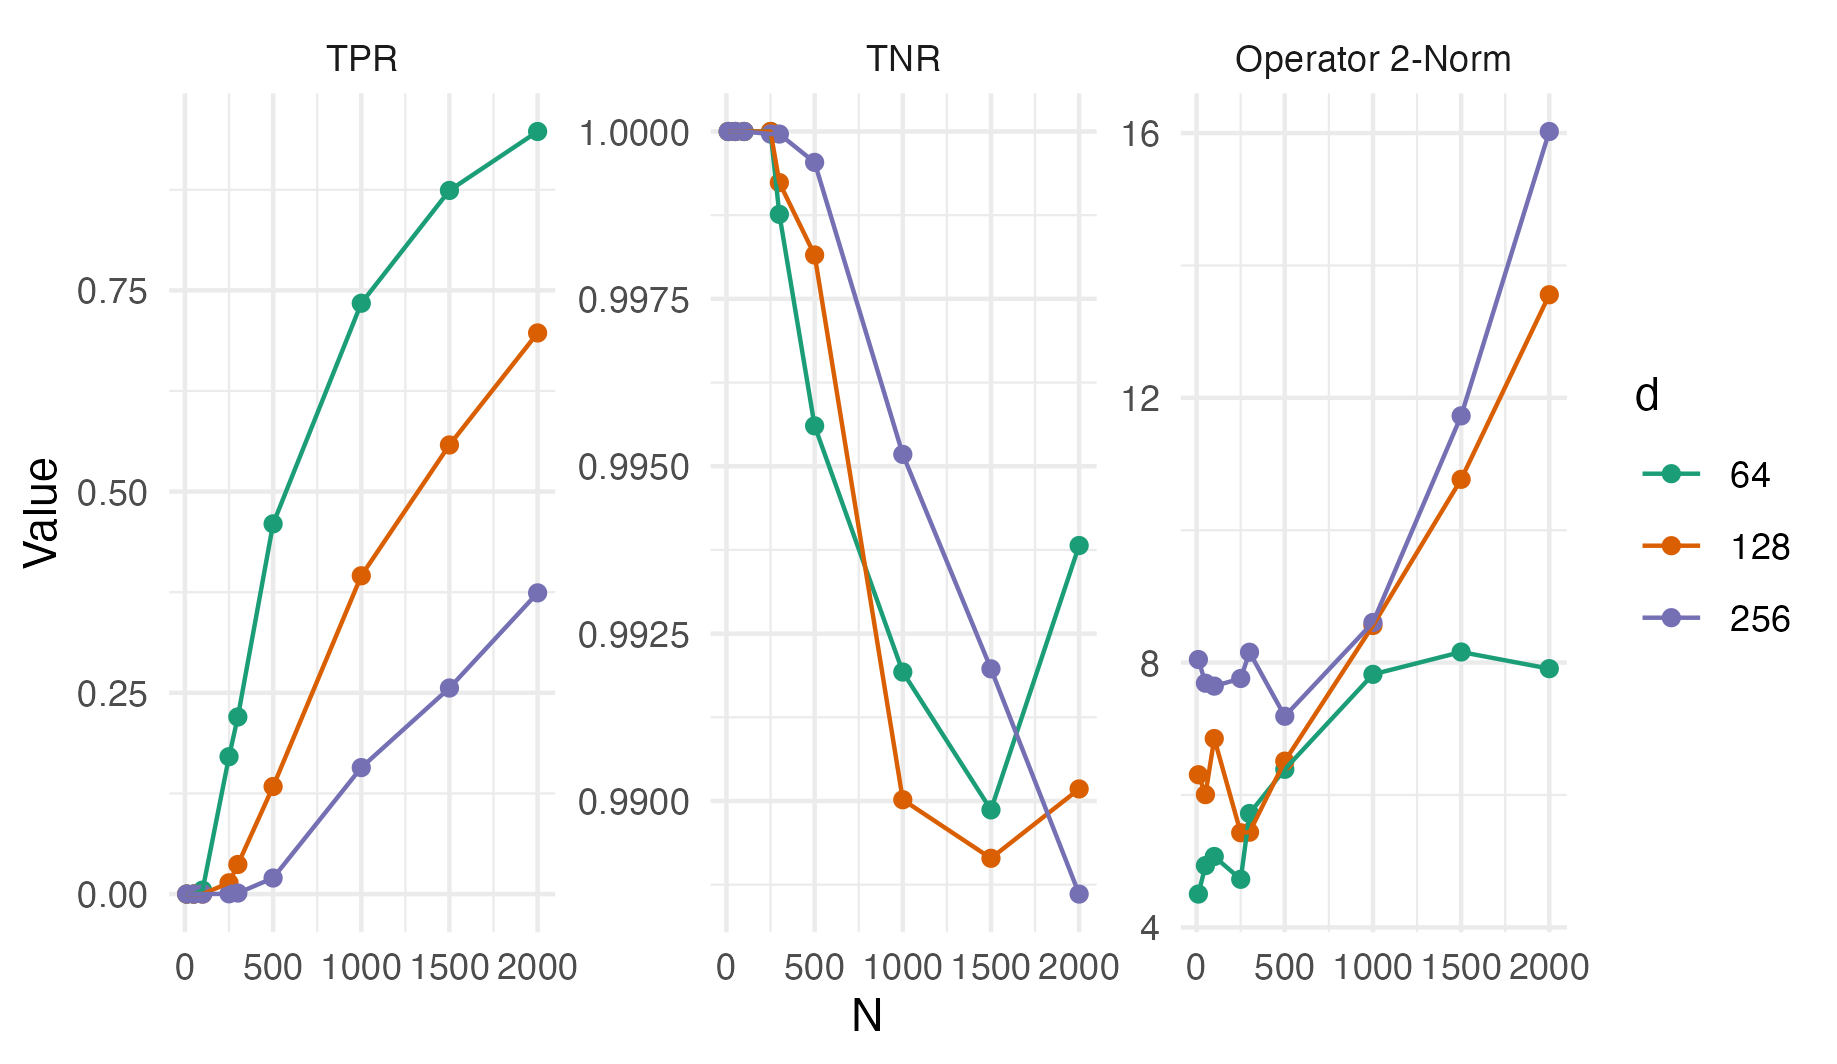
\includegraphics[scale=0.65]{glasso_complete_ERmb_FixN_2.png}
        \caption{ER(0.2), $\rho=0.4$ adjacency structure}
    \end{figure}
\end{frame}



\begin{frame}{}
    \bf{\Large Misc. Notes}    
\end{frame}
    
\begin{frame}{Forgoing Sparsity Assumptions}
\begin{itemize}
\item In the above methods, we have almost uniformly assumed some sparsity and applied a penalty ($\ell_1$)
    \begin{enumerate}
        \item How often is this a viable assumption? 
        \item What do we do (or what happens) if we don't meet this sparsity requirement, more severely than our AR($\cdot)$ extension sims?  
    \end{enumerate}
\item     Mazumder (2012) \cite{mazumder_graphical_2012} offers an updated algorithm and insight into performance for $p$ close to but larger than $N$
\item Interplay between $d, N$, and graph-connectedeness affect computation time and convergence 
\end{itemize}
\end{frame}

\begin{frame}{Time-Series Data}

\begin{itemize} \setlength\itemsep{5mm}

    \item Consider that our repeated observations are time-indexed:
    \begin{itemize} 
        \item  $\{X_j(t), t \in \mathcal{T}, j=1, ..., N\}, X_j \in \mathbb{R}^d$ 
    \end{itemize}

    \item Graphical perspective of vector auto-regressive models
    \begin{itemize}
        \item $X_d(t) = \varepsilon_d(t) + \sum_{j\neq d}\sum_{t\in\mathcal{T}} \alpha_tX_j(t)$
    \end{itemize}


    \item Can infer "Granger causal" relationships
        \begin{itemize}
            \item Causal relationships for some time-series using prior data from a {\it different time series}
        \end{itemize}

\end{itemize}

See Michael Eichler's {\it "Granger-causality graphs for multivariate time series"} (2007) and Dahlhaus's and Eichler's (2003) {\it "Causality and graphical models in time series"} for further discussion  

\end{frame}


\begin{frame}{Inference with Debiased Lasso}
    \begin{itemize}
    \item The typical lasso estimator $\hat\beta_\lambda = \text{argmin}\beta ||Y-X\beta||_2^2 + \lambda||\beta||_1$ is biased for true $beta^*$
    \item Can construct debiased estimator $\hat\beta_\lambda^d$ with asymptotic normality 
    \item What inference does this permit in graphical models that use $\ell_1$ penalization? 
    \end{itemize}
\end{frame}



\begin{frame}{"Nothing new under the sun"}
    My (likely useless and certaintly non-falsifiable) conspiracy theory: Did Euler {\it really} originate graph theory? For how intuitive graphs seem to understanding interrelationships, this much have existed in some primitive form? Or for how financially relevant this seems, I'm sure some BCE gambler had an idea of "interconnectedness"\newline \\ 
    For our historical blinders, see Babylonian and Chinese origins of the Pythagorean Theorem \newline \\ 
    Thoughts, possible leads? Let me know!
\end{frame}
\end{document}